\chapter{Анализ предметной области}

\section{Основные понятия}

\textbf{Управление памятью} \cite{glossary} --- это процесс координации и контроля использования памяти в вычислительной системе. Управление памятью выполняется на трёх уровнях. 

\begin{enumerate}[label*=\arabic*.]
	\item Аппаратное обеспечение управления памятью (MMU, ОЗУ и т.д.).
	\item Управление памятью операционной системы (виртуальная память, защита).
	\item Управление памятью приложения (выделение и освобождение памяти, сборка мусора).
\end{enumerate}

Аппаратное обеспечение управления памятью состоит из электронных устройств и связанных с ними схем, которые хранят состояние вычислительной системы. К этим устройствам относятся регистры процессора, кэш, ОЗУ, MMU (Memory Management Unit, блок управления памятью) и вторичная (дисковая) память. Конструкция запоминающих устройств имеет решающее значение для производительности современных вычислительных систем. Фактически пропускная способность памяти является основным фактором, влияющим на производительность системы. \cite{glossary}

Далее будет рассмотрено подробно управление памятью с точки зрения операционной системы и приложений.



\section{Управление памятью с точки зрения операционной системы}

\subsection{Иерархия памяти}

В процессе развития аппаратного обеспечения была разработана концепция \textbf{иерархии памяти}, согласно которой компьютеры обладают несколькими мегабайтами очень быстродействующей, дорогой и энергозависимой кэш-памяти, несколькими гигабайтами памяти, средней как по скорости, так и по цене, а также несколькими терабайтами памяти на довольно медленных, сравнительно дешевых дисковых накопителях, не говоря уже о сменных накопителях, таких как DVD и флеш-устройства USB. Превратить эту иерархию в абстракцию, то есть в модель, а затем управлять этой абстракцией --- и есть задача операционной системы. Та часть операционной системы, которая управляет иерархией памяти (или ее частью), называется \textbf{менеджером}, или \textbf{диспетчером}, \textbf{памяти} \cite{tannenbaum}. Он должен следить за тем, какие части памяти используются, выделять память процессам, которые в ней нуждаются, и освобождать память, когда процессы завершат свою работу. Выбор, совершаемый менеджером памяти на этом этапе, может оказать существенное влияние на будущую эффективность программы, так как до 40\% (в среднем 17\%) времени её выполнения затрачивается на выделение и освобождение памяти. \cite{cornell}

\subsection{Адресное пространство процесса}

Чтобы допустить одновременное размещение в памяти нескольких приложений без создания взаимных помех, нужно решить две проблемы, относящиеся к защите и перемещению. Так была разработана новая абстракция операционной системы --- адресное пространство. Так же, как понятие процесса создает своеобразный абстрактный центральный процессор для запуска программ, понятие адресного пространства создаёт своеобразную абстрактную память, в которой существуют программы. \textbf{Адресное пространство} \cite{tannenbaum} --- это набор адресов, который может быть использован процессом для обращения к памяти. У каждого процесса имеется собственное адресное пространство, независимое от адресных пространств других процессов (за исключением тех случаев, когда процессам требуется совместное использование их адресных пространств).

В каждой операционной системе может по-разному задаваться структура адресного пространства процесса, но, как правило, она содержит две концептуальные области: стек и кучу. \textbf{Стек} \cite{windows} --- область адресного пространства процесса, предназначенная для хранения параметров функций, локальных переменных и адреса возврата после вызова функции. \textbf{Куча} \cite{linux} --- область адресного пространства процесса, предназначенная для выделения памяти, динамически запрашиваемой программой.

\subsection{Виртуальная память}

Для обеспечения одновременного содержания в памяти множества процессов были выработаны два основных подхода. Самый простой из них, называемый \textbf{свопингом}, заключается в размещении в памяти всего процесса целиком, его запуске на некоторое время, а затем сбросе на диск. Бездействующие процессы большую часть времени хранятся на диске и в нерабочем состоянии не занимают пространство оперативной памяти (хотя некоторые из них периодически активизируются, чтобы проделать свою работу, после чего опять приостанавливаются). Второй подход называется \textbf{виртуальной памятью}, он позволяет программам запускаться даже в том случае, если они находятся в оперативной памяти лишь частично.

\textbf{Виртуальная память} --- метод управления оперативной (внутренней) памятью компьютера, позволяющий выполнять программы, требующие больше оперативной памяти, чем имеется в компьютере, путём автоматического перемещения частей программы между оперативной памятью и вторичным хранилищем (файл на диске или раздел подкачки). В основе виртуальной памяти лежит идея о том, что у каждой программы имеется собственное адресное пространство, которое разбивается на участки, называемые \textbf{страницами} \cite{tannenbaum}. Каждая страница представляет собой непрерывный диапазон адресов. Эти страницы отображаются на физическую память, но для запуска программы одновременное присутствие в памяти всех страниц необязательно.

Если программа требует больше памяти, чем есть в распоряжении компьютера, то операционная система в соответствии с \textbf{алгоритмом замещения страниц} \cite{tannenbaum} выбирает страницы, которые выгружаются из оперативной памяти. Освобождённая оперативная память отдаётся другой программе, которая её запросила. В дальнейшем, если к выгруженной странице произойдёт обращение, операционная система выберет страницу для выгрузки из памяти, чтобы освободить место для загружаемой страницы.

Подмножество виртуального адресного пространства процесса, находящееся в физической памяти, называется \textbf{рабочим набором}. \cite{windows}

% Одной из задач распределения памяти является вычисление адресов для фрагментов программы и информационных объектов, исходя из фиксируемого при генерации взаимного их расположения, причем для адресов тех объектов, расположение которых в памяти нельзя определить статически (при трансляции), генерируются динамические вычисления этих адресов.

\subsection{Функции операционной системы по управлению памятью}

Помимо первоначального выделения памяти процессам при их создании операционная система должна также заниматься динамическим распределением памяти, то есть обслуживать запросы приложений на выделение им дополнительной памяти во время выполнения. После того, как приложение перестаёт нуждаться в дополнительной памяти, оно может вернуть её системе. Выделение случайного объёма памяти в случайные моменты времени из общего пула приводит к фрагментации памяти и, вследствие этого, к неэффективному её использованию. Дефрагментация памяти также является функцией операционной системы.

Таким образом, можно сформулировать следующие функции ОС по управлению памятью в мультипрограммных системах.

\begin{enumerate}[label*=\arabic*.]
	\item Отслеживание свободной и занятой памяти.
	\item Управление виртуальными адресными пространствами процессов, в том числе отображение виртуального адресного пространства процесса на физическую память.
	\item Динамическое распределение памяти. 
	\item Дефрагментация памяти. 
\end{enumerate}



\section{Управление памятью с точки зрения приложений}

\subsection{Среда выполнения языка программирования}

Менеджер памяти операционной системы с точки зрения выполняющихся на ней приложений обладает двумя серьёзными недостатками. Во-первых, он является недетерминированным: процессы не могут напрямую влиять на решения, принимаемые операционной системой по управлению их адресными пространствами. Во-вторых, Менеджер памяти операционной системы не реализует те функции управления памятью, которые требуются конечному пользователю. Поэтому языки программирования реализуют собственную \textbf{среду выполнения} (language runtime), в которой реализуют необходимые пользователю функции для работы с памятью и создают собственные абстракции памяти.

Среда выполнения языка программирования может выполнять следующие функции: \cite{dotnet_clr}

\begin{enumerate}[label*=\arabic*)]
	\item управление памятью;
	\item обработка исключений; 
	\item сборка мусора; 
	\item контроль типов;
	\item обеспечение безопасности; 
	\item управление потоками. 
\end{enumerate}

Управление потоками в среде выполнения языка подразумевает, что язык программирования организует многопоточное выполнение программы, используя возможности операционной системы, а также реализует некоторую \textbf{модель памяти}, которая для императивных языков программирования, поддерживающих многопоточное выполнение, определяет, какие записи в разделяемые переменные могут быть видны при чтениях, выполняемых другими потоками. \cite{memory_model}

\subsection{Управление памятью}
\label{memory_management}

Менеджер памяти приложения должен учитывать следующие ограничения. \cite{mm_overview}

\begin{enumerate}[label*=\arabic*.]
	\item \textbf{Нагрузка на процессор} --- дополнительное время, затрачиваемое диспетчером памяти во время работы программы.
	\item \textbf{Блокировки} --- время, необходимое диспетчеру памяти для завершения операции и возврата управления программе. Это влияет на способность программы оперативно реагировать на интерактивные события, а также на любое асинхронное событие, например связанное с сетевым взаимодействием.
	\item \textbf{Накладные расходы памяти} --- дополнительный объём памяти, затрачиваемый на администрирование, а также накладные расходы, связанные с внутренней и внешней фрагментацией. \textbf{Внутренняя фрагментация} \cite{glossary} --- явление, при котором аллокатор выделяет при каждом запросе больше памяти, чем фактически запрошено. \textbf{Внешняя фрагментация} \cite{glossary} --- явление, при котором свободная память разделена на множество мелких блоков, ни один из которых нельзя использовать для обслуживания запроса ан выделение памяти.
\end{enumerate}

Основная проблема управления памятью состоит в том, чтобы понять, когда следует сохранить содержащиеся в ней данные, а когда их следует уничтожить, чтобы память можно было использовать повторно. К сожалению, существует множество способов, которыми плохая практика управления памятью может повлиять на надежность и быстродействие программ, как при ручном, так и при автоматическом управлении памятью.

Ниже перечислены наиболее частые проблемы управления памятью. \cite{mm_overview}

\begin{enumerate}[label*=\arabic*.]
	\item \textbf{Преждевременное освобождение памяти} (premature free). 
	Когда программы освобождают память, но позже пытаются получить к ней доступ, их поведение становится неопределённым. Сохранившаяся ссылка на освобождённую память называется \textbf{висячим указателем} (dangling pointer).
	\item \textbf{Утечки памяти} (memory leaks). Когда программы интенсивно выделяют память, не освобождая её, в конечном итоге память заканчивается.
	\item \textbf{Внешняя фрагментация} (external fragmentation). Работа аллокатора по выделению и освобождению памяти может привести к тому, что он больше не сможет выделять достаточно большие области памяти, несмотря на наличие достаточного общего количества свободной памяти. Это связано с тем, что свободная память может быть разделена на множество небольших областей, разделённых используемыми данными. Данная проблема особенно критична в серверных приложениях, работающих в течение длительного времени.
	\item \textbf{Неэффективное расположение ссылок} (poor locality of reference). Эта проблема связана с тем, как современные менеджеры памяти аппаратного обеспечения и операционной системы обращаются с памятью: последовательные обращения к памяти выполняются быстрее, если они производятся к соседним областям памяти. Если менеджер памяти разместит данные, которые программа будет использовать вместе, не в соседних областях памяти, то быстродействие программы уменьшится.
	\item \textbf{Негибкий дизайн} (inflexible design). Менеджеры памяти могут вызвать серьезные проблемы с производительностью, если они были разработаны с одной целью, а используются для другой. Эти проблемы вызваны тем, что любое решение по управлению памятью опирается на предположения о том, как программа будет использовать выделенную память. Например, на стандартные размеры областей памяти, шаблоны ссылок или время жизни объектов. Если эти предположения неверны, то диспетчер памяти может работать с памятью менее эффективно.
	\item \textbf{Межмодульное взаимодействие} (interface complexity). Если объекты передаются между модулями программы, то при проектировании интерфейсов модулей необходимо учитывать управление их памятью.
\end{enumerate}

Управление памятью приложения объединяет две взаимосвязанные задачи: выделение памяти (allocation) и её переиспользование (recycling), когда она больше не требуется. За выделение памяти отвечает \textbf{аллокатор} \cite{allocator}. Его необходимость обусловлена тем, что процессы, как правило, не могут заранее предсказать, сколько памяти им потребуется, поэтому они нуждаются в реализации дополнительной логики обслуживания изменяющихся запросов к памяти. Решение об освобождении и переиспользовании выделенной аллокатором памяти, которая больше не используется приложением, может быть принято либо программистом, либо средой выполнения языка. Соответственно, в зависимости от этого управление памятью в языке программирования может считаться либо ручным, либо автоматическим.

\subsubsection{Ручное управление памятью}

При ручном управлении памятью программист имеет прямой контроль над временем жизни объектов программы. Как правило, он осуществляется либо явными вызовами функций управления кучей (например, malloc и free в C), либо языковыми конструкциями, влияющими на стек управления (например, объявлениями локальных переменных). Ключевой особенностью ручного менеджера памяти является то, что он даёт возможность явно указать, что заданная область памяти может быть освобождена и переиспользована. \cite{mm_overview}

Преимущества ручного управления памятью: 

\begin{itemize}[label*=---]
	\item явное выделение и освобождение памяти делает программы более прозрачными для разработчика;
	\item ручные менеджеры памяти, как правило, используют память более экономно, так как программист может минимизировать время между моментом, когда выделенная память перестаёт использоваться, и её фактическим освобождением.
\end{itemize}

Недостатки ручного управления памятью: 

\begin{itemize}[label*=---]
	\item увеличение исходного кода программ за счёт того, что управление памятью, как правило, составляет значительную часть интерфейса любого модуля;
	\item повышение дублирования кода за счёт использования однотипных инструкций управления памятью;
	\item увеличение числа ошибок управления памятью из-за человеческого фактора.
\end{itemize}

К языкам с ручным управлением памятью относятся C, C++, Zig и другие. На таких языках программисты могут писать код, дублирующий поведение менеджера памяти либо путем выделения больших областей и их разделения для использования, либо путем внутреннего переиспользования этих блоков. Такой код называется \textbf{субаллокатором} (suballocator) \cite{glossary}, так как он работает поверх другого аллокатора. Субаллокаторы могут использовать как преимущество специальные знания о поведении программы, но в целом они менее эффективны, чем использование базового аллокатора. Также стоит отметить, что субаллокаторы могут быть неэффективными или ненадежными, тем самым создавая новый источник ошибок. \cite{allocator}



\subsubsection{Автоматическое управление памятью}

Автоматическое управление памятью \cite{mm_overview} --- это служба, которая автоматически перерабатывает память, которую программа не собирается использовать в дальнейшем. Эта служба, как правило, работает либо как часть среды выполнения языка, либо как расширение. Автоматические менеджеры памяти обычно перерабатывают области памяти, которые недоступны из переменных программы (то есть области, к которым невозможно получить доступ с помощью указателей). Автоматическая переработка динамически выделяемой памяти называется \textbf{сборкой мусора}. Термин <<мусор>> используется для обозначения объектов, о которых достоверно известно, что они не используются программой, так являются недостижимыми из других её объектов. Термин <<недостижимость>> может иметь различные интерпретации в разных языках программирования. \cite{glossary}

Задачи автоматического управления памятью: 

\begin{itemize}[label*=---]
	\item выделение памяти под новые объекты;
	\item идентификация используемых объектов;
	\item освобождение памяти, занятой неиспользуемыми объектами.
\end{itemize}

Преимущества автоматического управления памятью: 

\begin{itemize}[label*=---]
	\item освобождение разработчика от задачи управления памятью в своих программах;
	\item уменьшение объёма исходного программ за счёт отсутствия необходимости явно работать с памятью;
	\item уменьшение числа ошибок управления памятью;
	\item автоматическое управление памятью может быть более эффективным, чем ручное, за счёт применения соответствующих алгоритмов.
\end{itemize}

Недостатки автоматического управления памятью: 

\begin{itemize}[label*=---]
	\item время жизни объектов программы становится непрозрачным для разработчика, так как часть логики работы с памятью реализована на уровне языка;
	\item память, как правило, используется менее экономно, так как существует некоторая задержка между моментом, когда память перестаёт использоваться, и моментом её освобождения; такие задержки определяются алгоритмами автоматической переработки памяти.
\end{itemize}

Автоматическое управление памятью используется в большинстве современных языков программирования, среди которых C\#, Golang, Haskell, Java, JavaScript, Python, Swift, частично Rust, C++ при использовании умных указателей и другие. Как правило, в таких языках автоматическая сборка мусора реализуется либо методом подсчёта ссылок, либо с использованием отслеживающего сборщика мусора. \cite{recycling} Стоит отметить, что для автоматического управления памятью также можно использовать гибридные методы. \cite{cornell2} \cite{urc}

В языках с автоматическим управлением памятью часто необходимо выполнять действия над некоторыми объектами после того, как они перестали использоваться, и до того, как память, которую они занимают, может быть переиспользована. Такие действия называются \textbf{финализаторами}, а их выполнение --- \textbf{финализацией} (finalization, termination). \cite{glossary}

Как правило, финализация используется для освобождения ресурсов, когда работающий с ними объект перестаёт использоваться. Например, открытый файл может быть представлен объектом потока ввода-вывода. Когда менеджер памяти подтверждает, что этот объект больше не используется в программе, то можно быть гарантировать, что файл больше не используется программой и его нужно закрыть до повторного использования потока. \cite{glossary}

Стоит отметить, что момент финализации объекта программы, как правило, не фиксирован. Этот факт может стать проблемой, если финализация используется для управления ограниченными ресурсами операционной системы, такими как файловые дескрипторы. \cite{glossary}



\subsection{Трассирующая сборка мусора}
\label{roots}

\textbf{Сборщик мусора} \cite{glossary} --- автоматический менеджер памяти, реализующий некоторый алгоритм сборки мусора.

\textbf{Трассирующий сборщик мусора} \cite{recycling} --- автоматический менеджер памяти, который следует указателям, чтобы определить, какие области памяти доступны из переменных программы, называемых \textbf{корневым набором}).

Целью идеального сборщика мусора является освобождение пространства, используемого каждым объектом, как только он перестаёт использоваться программой.

Далее будут подробно рассмотрены основные алгоритмы сборки мусора. Стоит отметить, что алгоритмы могут сочетаться и заменяться во время выполнения программы в зависимости от параметров кучи, таких ка заполненность и фрагментация. \cite{handbook}

\subsubsection{Трёхцветная абстракция}
\label{tricolor}

Для разработки и описания алгоритмов сборки мусора важно иметь краткий способ описания состояния объектов во время сборки (были ли они помечены, есть ли они в рабочем списке и так далее). Трёхцветная абстракция позволяет трассирующим сборщикам мусора судить о корректности сборки в терминах инвариантов, которые сборщики должны сохранять. В рамках трехцветной абстракции трассирующий сборщик мусора разбивает граф объектов на черные (предположительно используемые) и белые (возможно, неиспользуемые) объекты. Изначально каждый объект белый. Когда объект впервые обнаруживается во время трассировки, он окрашивается в серый цвет. Когда объект был отсканирован и были идентифицированы его дочерние элементы, он закрашивается черным. Концептуально объект является черным, если сборщик завершил его обработку, и серым, если сборщик знает о нем, но еще не закончил его обработку (или должен обработать его снова). По аналогии с цветом объекта, полям также может быть присвоен цвет: серый, когда сборщик впервые сталкивается с ними, и черный, когда он обработал их. Трассировка выполняется по всей куче путём перемещения волнового фронта сборщика мусора (серые объекты), отделяющего чёрные объекты от белых до тех пор, пока все доступные объекты не будут окрашены чёрным цветом. \cite{handbook}

\begin{figure}[H]
	\centering
	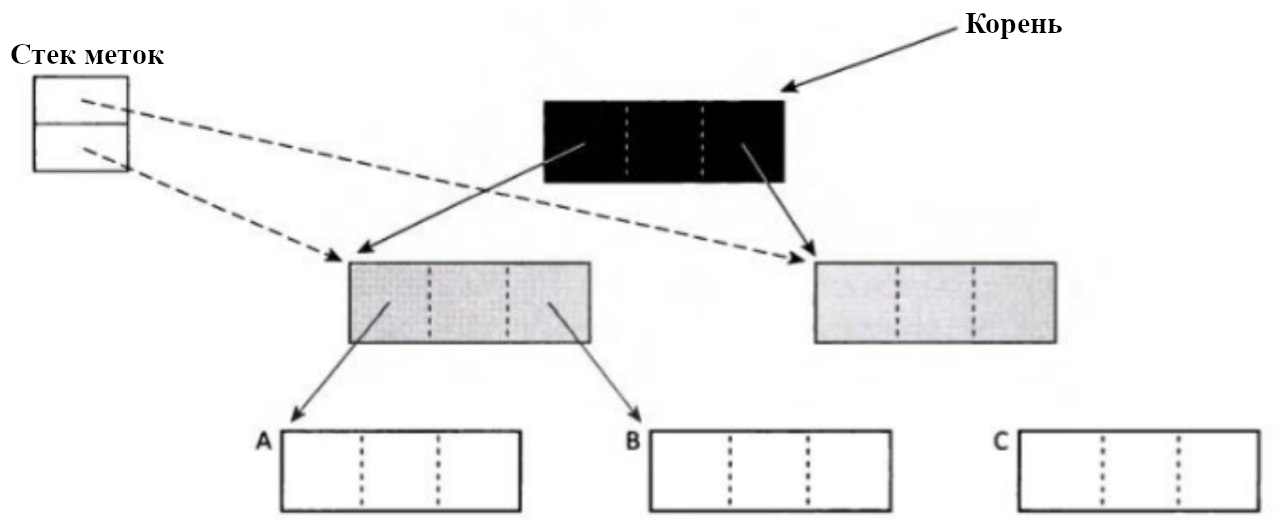
\includegraphics[width=\textwidth]{assets/tricolor.png}
	\caption{Пример трёхцветной разметки}
	\label{fig:tricolor}
\end{figure}

На рисунке \ref{fig:tricolor} показан пример разметки графа объектов и стек меток, реализующий рабочий список, в процессе работы сборщика мусора. Все объекты, хранящиеся в стеке меток, будут посещены, поэтому они окрашиваются в серый цвет. Любой объект, который был размечен и не находится в стеке, является чёрным (корень графа на рисунке), а все остальные объекты окрашиваются в белый цвет (в настоящее время A, B и C). Однако, как только разметка графа завершится, стек меток будет пуст (без серых объектов) и только C останется белым (мусор), а все остальные объекты будут окрашены чёрным.

Алгоритм сохраняет важный инвариант: в конце каждой итерации цикла разметки отсутствуют ссылки с чёрных объектов на белые. Таким образом, любой доступный белый объект должен быть доступен из серого объекта. Если бы этот инвариант был нарушен, то используемый потомок чёрного объекта мог быть окрашен белым (и, следовательно, был бы освобожден некорректно), поскольку сборщик не обрабатывает чёрные объекты дальше. Трехцветное представление состояния объектов программы особенно полезно при рассмотрении алгоритмов параллельной сборки мусора, когда она выполняется конкурентно с потоками основной программы. \cite{handbook}



\subsubsection{Алгоритм mark-sweep}
\label{mark-sweep}

Алгоритм mark-sweep реализует рекурсивное определение достижимости объекта по указателям. Сборка мусора осуществляется в два этапа. Сначала сборщик обходит граф объектов, начиная с <<корней>> (регистры, стеки потоков, глобальные переменные), через которые программа могла бы немедленно получить доступ к объектам, а затем, следуя указателям, сканирует каждый найденный объект. Такой обход называется \textbf{трассировкой}. На втором этапе, этапе очистки (sweep), сборщик проверяет каждый объект в куче: любой неразмеченный объект считается мусором и освобождается. \cite{handbook}

Mark-sweep --- это алгоритм косвенного сбора данных. В отличие от косвенных методов, прямые алгоритмы, такие как подсчёт ссылок, определяют достижимость объекта исключительно по самому объекту, без обращения к трассировке.  \cite{handbook}

Рассматриваемый алгоритм не обнаруживает мусор как таковой, а скорее идентифицирует все используемые объекты, а затем приходит к выводу, что всё остальное должно быть мусором. Стоит заметить, что сборщику необходимо размечать используемые объекты при каждом вызове. Для обеспечения согласованности при работе с памятью сборщик мусора, реализующий алгоритм mark-sweep, не должен работать параллельно или конкуррентно с основной программой. Такой режим работы сборщика называют <<\textbf{остановкой мира}>> (<<stop the world>>). \cite{handbook}

На рисунках \ref{fig:mark-sweep-1}-\ref{fig:mark-sweep-3} представлены схемы алгоритма mark-sweep, использующего битовую карту размеченных областей кучи (bitmap). \cite{handbook}

\begin{figure}[H]
	\centering
	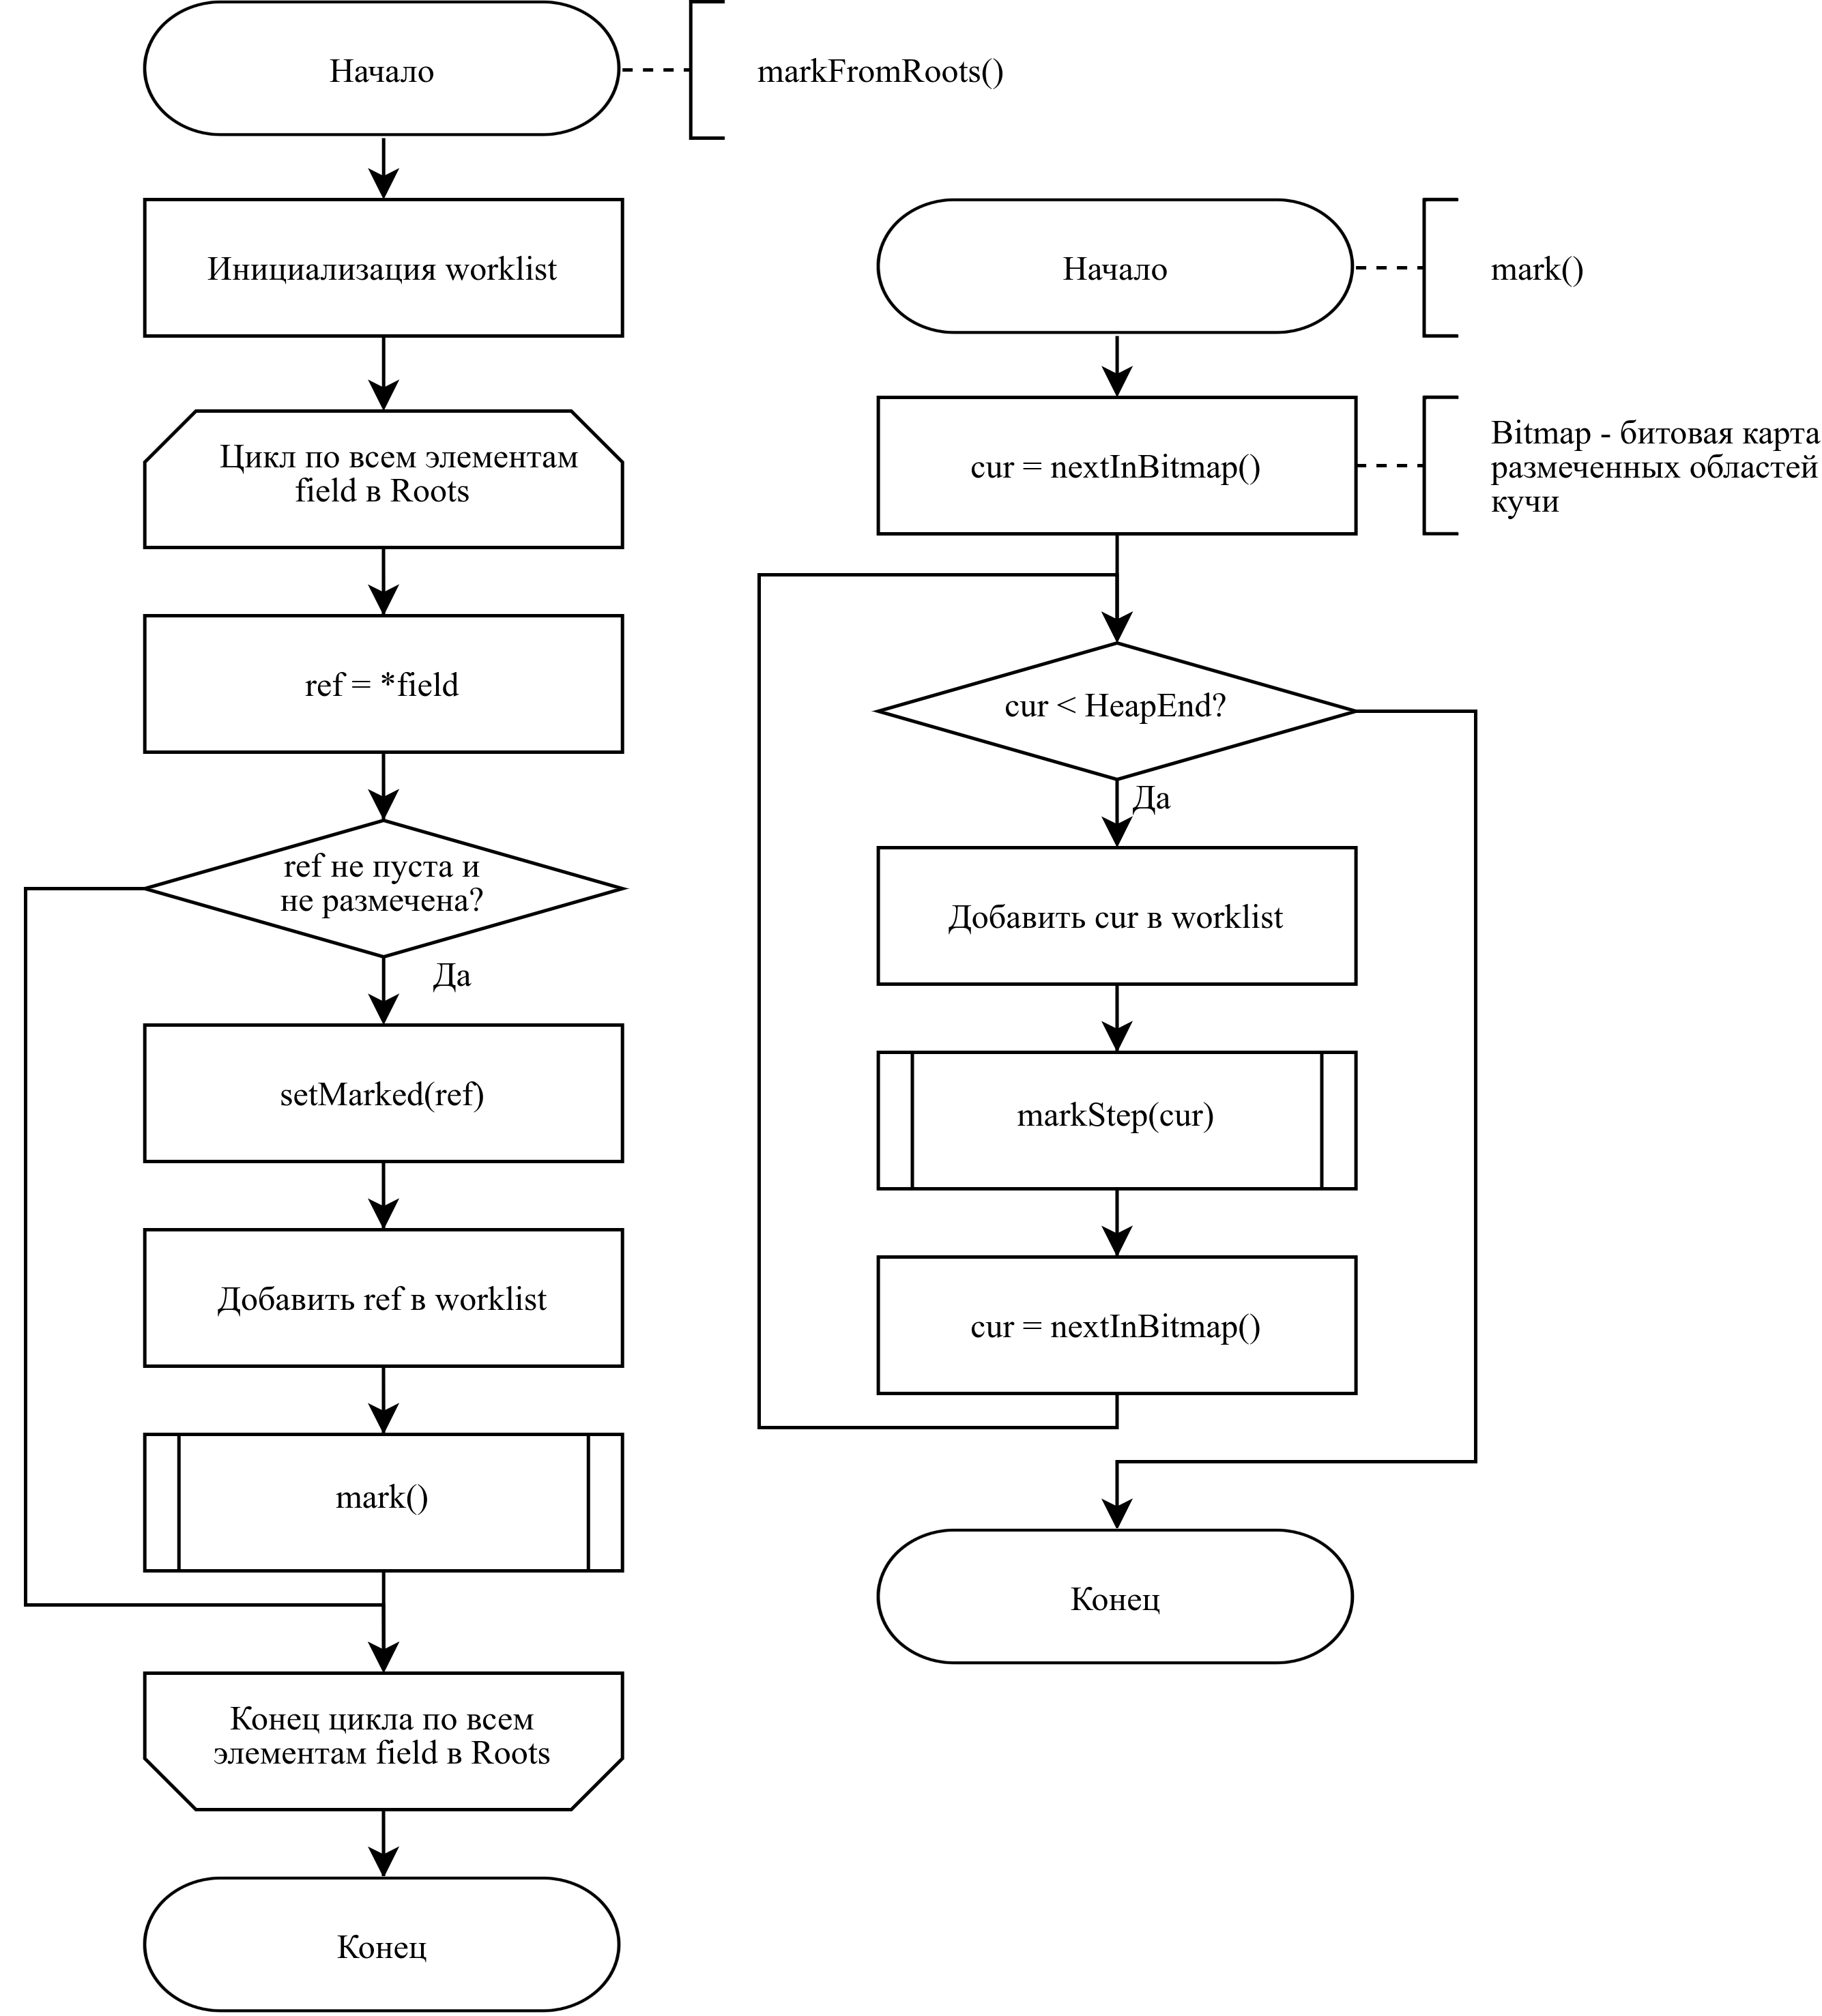
\includegraphics[scale=0.175]{assets/mark-sweep-1.png}
	\caption{Функции разметки объектов из корневого набора и рабочего списка}
	\label{fig:mark-sweep-1}
\end{figure}

\begin{figure}[H]
	\centering
	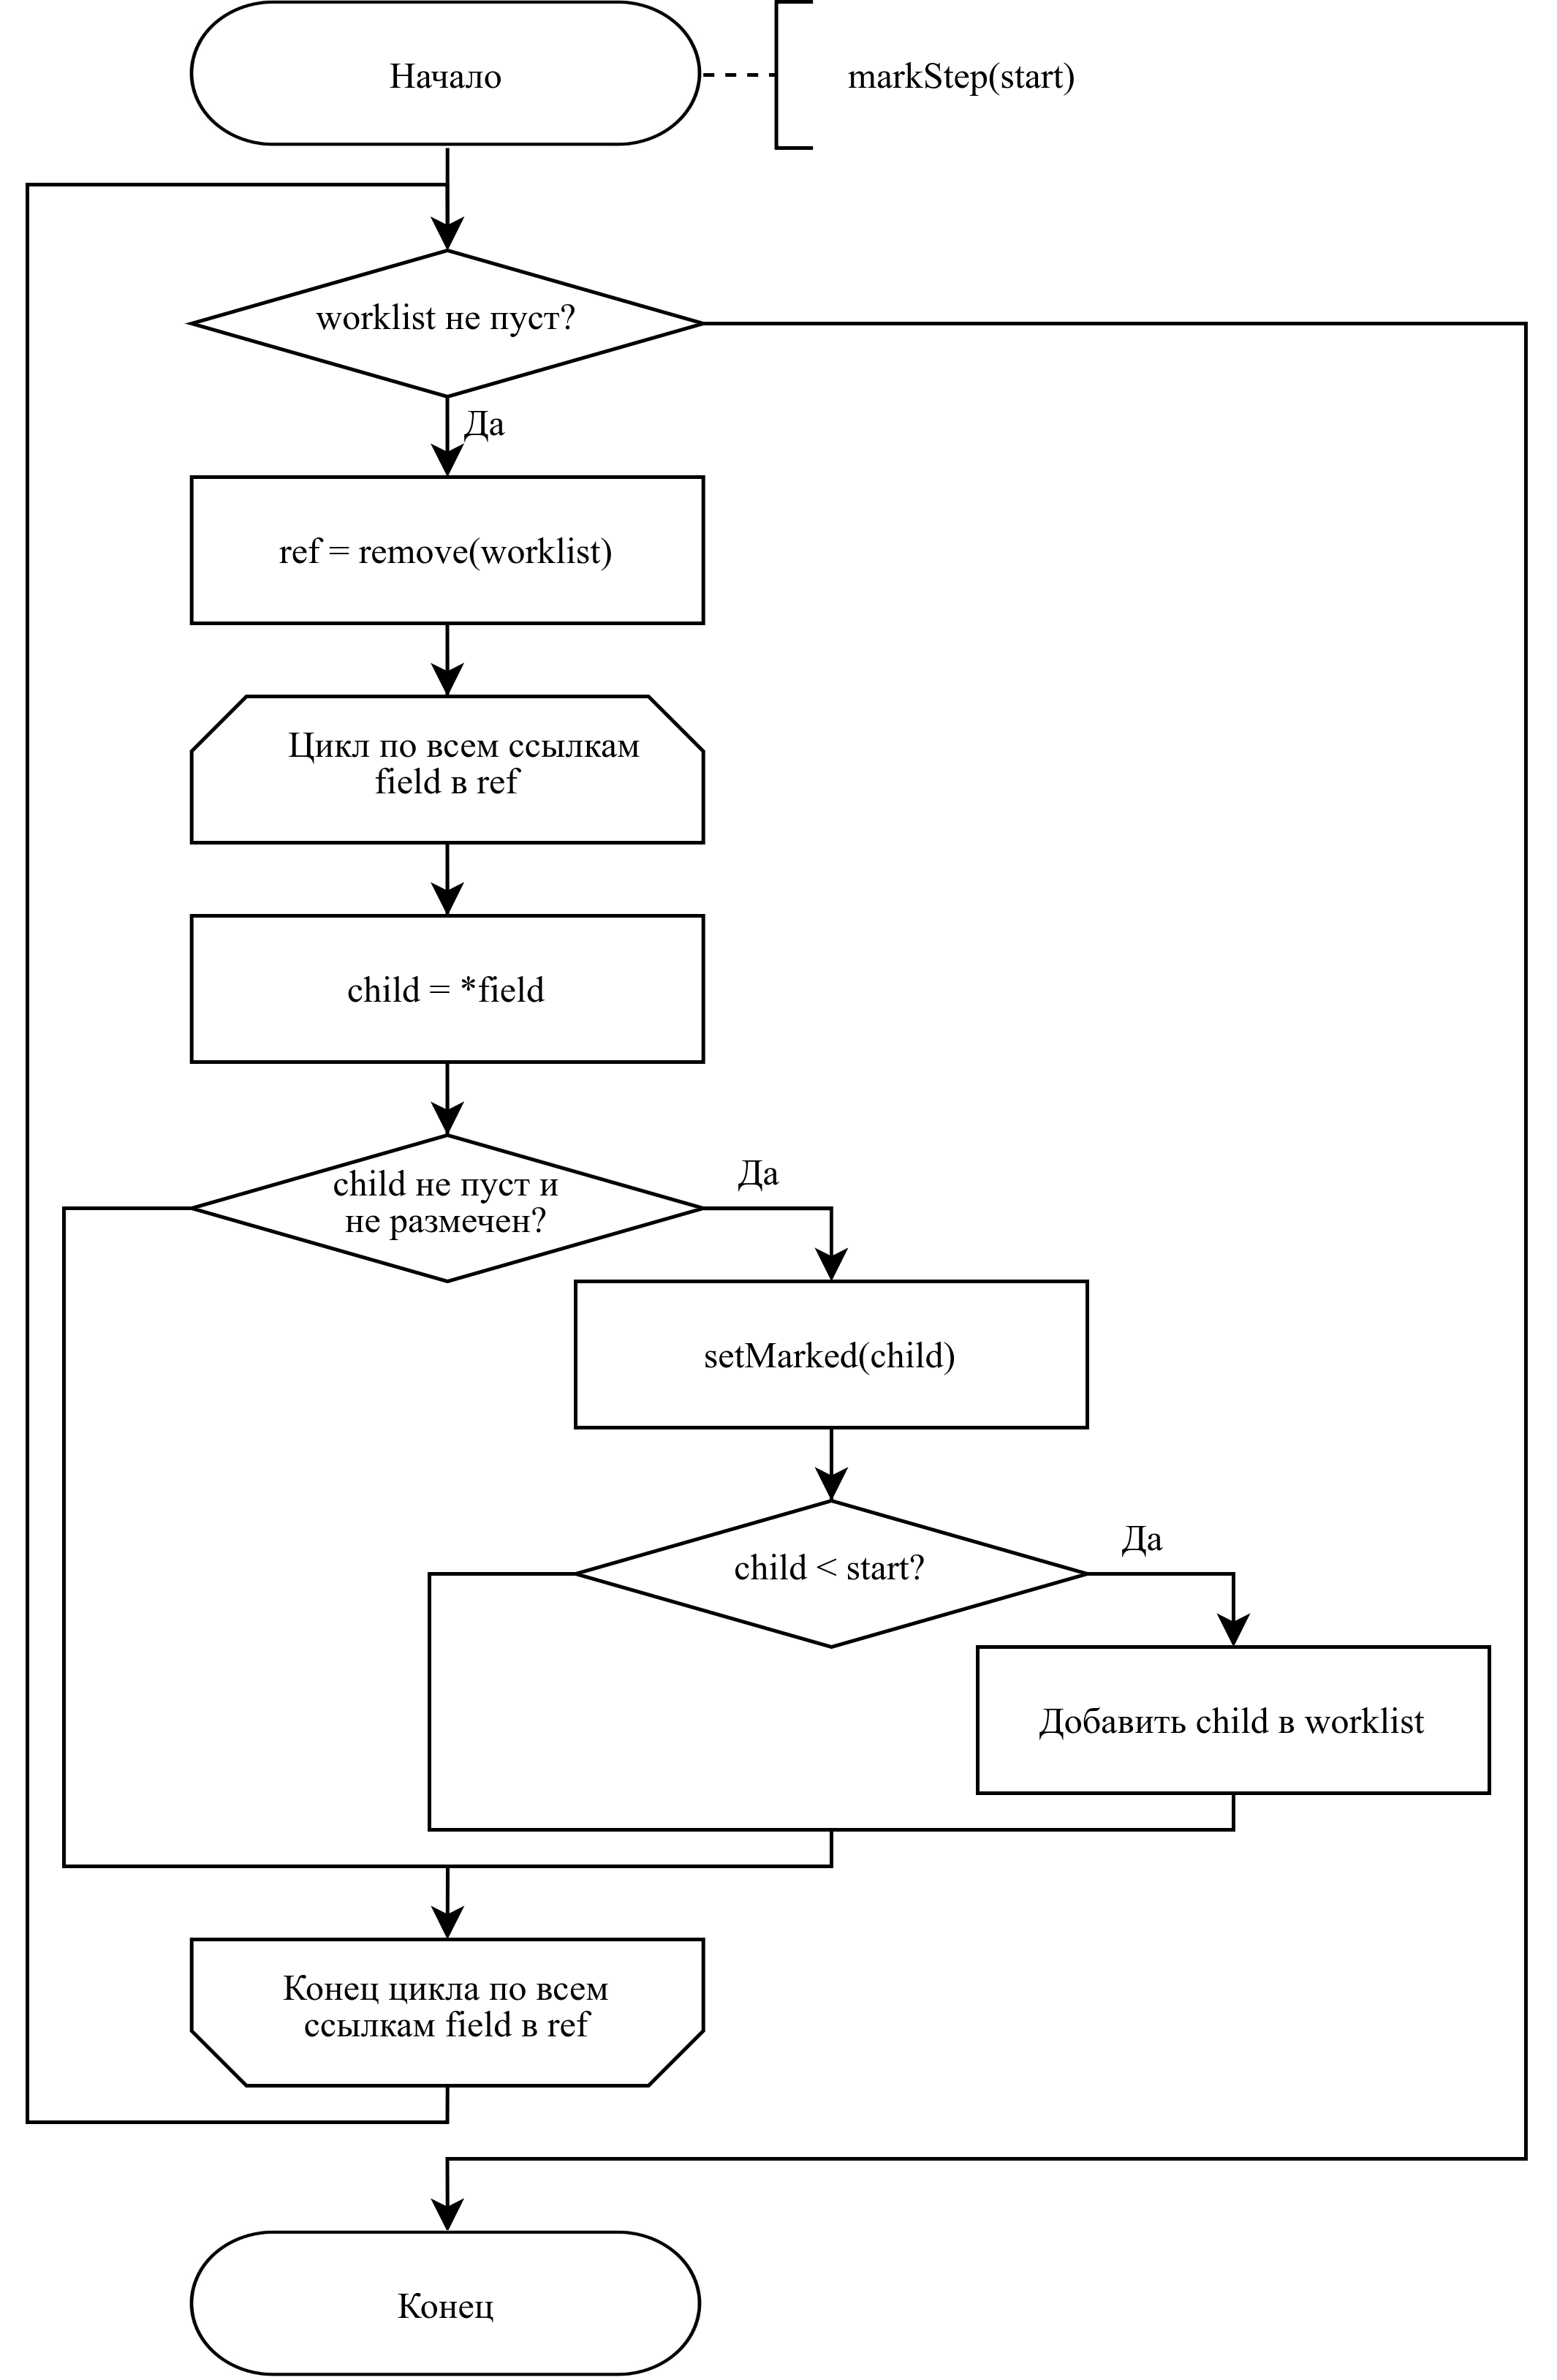
\includegraphics[scale=0.175]{assets/mark-sweep-2.png}
	\caption{Функция разметки одного объекта}
	\label{fig:mark-sweep-2}
\end{figure}

\begin{figure}[H]
	\centering
	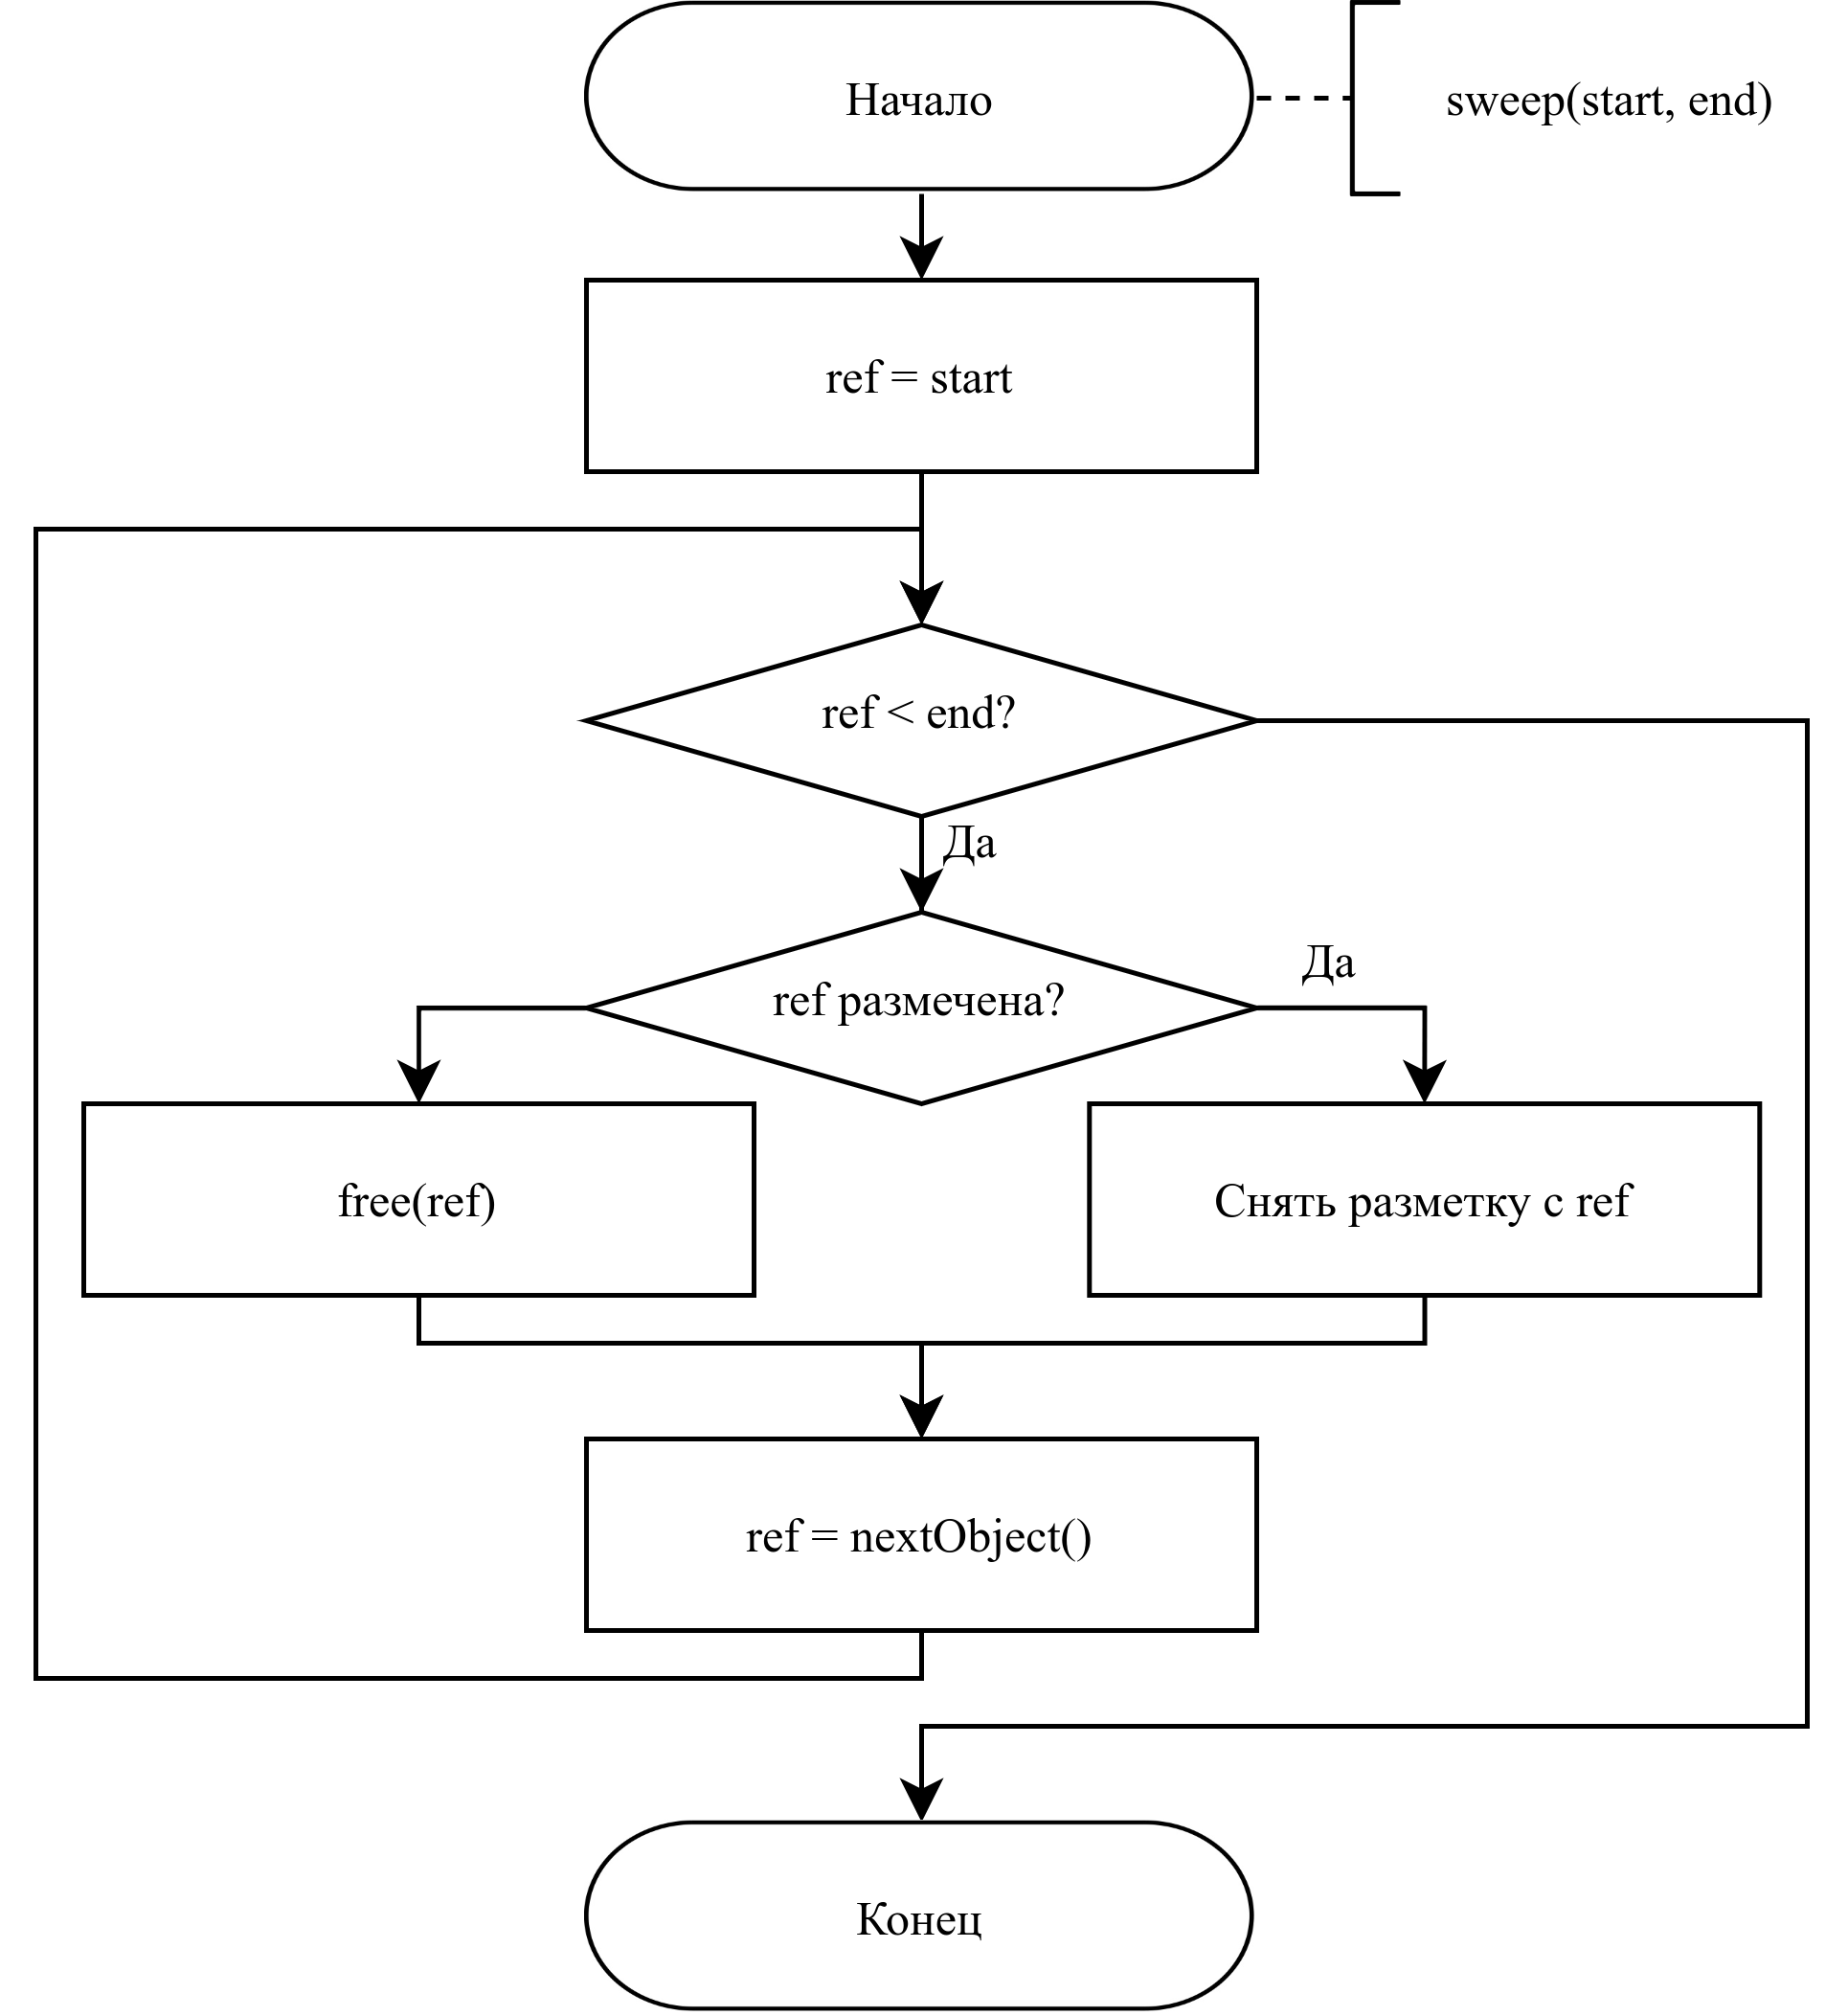
\includegraphics[scale=0.175]{assets/mark-sweep-3.png}
	\caption{Функция очистки}
	\label{fig:mark-sweep-3}
\end{figure}

Как и другие алгоритмы трассировки, алгоритм mark-sweep должен идентифицировать все используемые объекты в пространстве, прежде чем сможет освободить память, используемую любыми мусорными объектами. Это относительно дорогостоящая операция, поэтому её следует проводить как можно реже. Это означает, что трассирующим сборщикам мусора необходимо предоставить некоторый запас памяти для работы в куче. Если используемые объекты занимают слишком большую часть кучи, а аллокаторы выделяют память слишком быстро, то сборщик мусора, работающий по алгоритму mark-sweep, будет вызываться слишком часто и замедлять основную программу. Для обеспечения пропускной способности, сравнимой с той, что обеспечивается ручным управлением памятью, запас памяти в куче должен составлять не менее 20\%. \cite{handbook}

Как правило, в длительно работающих приложениях куча имеет тенденцию к фрагментации. Для неперемещающих аллокаторов требуется пространство, в O(log(max/min)) большее минимально возможного, где min и max --- наименьший и наибольший возможный размеры объекта. Таким образом, возможно, придется вызывать неуплотняющий сборщик мусора чаще, чем тот, который уплотняет используемые объекты. \cite{handbook}

Чтобы избежать снижения производительности из-за чрезмерной фрагментации, многие сборщики, использующие алгоритм mark-sweep для управления кучей, также периодически используют другой алгоритм, такой как mark-compact, для её дефрагментации. Такой подход особенно актуален, если приложение не поддерживает достаточно постоянные соотношения размеров объектов или выделяет много относительно больших объектов. Понизить склонность кучи к фрагментации также может помочь использование того факта, что объекты склонны к выделению и освобождению группами. Размещение объектов группами также может уменьшить необходимость в уплотнении кучи. \cite{handbook}



\subsubsection{Алгоритм mark-compact}
\label{mark-compact}

Фрагментация может быть проблемой для неперемещающих сборщиков мусора. Несмотря на то, что в куче может быть свободное пространство, либо может отсутствовать непрерывная область, достаточно большая для удовлетворения запроса на выделение памяти, либо время, затрачиваемое на выделение, может стать чрезмерным, поскольку менеджеру памяти приходится искать подходящее свободное пространство. Для борьбы с фрагментацией аллокаторы могут хранить небольшие объекты одинакового размера в смежных областях памяти. Это особенно актуально для приложений, которые не выделяют много относительно больших объектов.  \cite{handbook}

Однако многие длительно работающие приложения, управляемые неперемещающими сборщиками, будут фрагментировать кучу, что отрицательно скажется на производительности приложений. Для устранения внешней фрагментации предлагается две стратегии. Первая, которой придерживается алгоритм mark-compact, заключается в уплотнении используемых объектов кучи, вторая --- в перемещении объектов из одной области памяти в другую. Основное преимущество уплотнения кучи заключается в том, что она обеспечивает относительно быстрое последовательное распределение, просто проверяя ограничение кучи и находя свободный указатель, соответствующий запросу на выделение. \cite{handbook}

Алгоритм mark-compact работает в несколько этапов. Первая фаза --- фаза разметки. Затем дальнейшие
этапы уплотнения сжимают используемые данные путем перемещения объектов и обновления значений указателей всех ссылок на объекты, которые были перемещены. Количество обходов кучи, порядок, в котором они выполняются, и способ перемещения объектов могут зависеть от реализации. Порядок уплотнения влияет на местоположение данных. Сборщик может перемещать объекты в куче одним из трех способов. \cite{handbook}

\begin{itemize}[label*=---]
	\item произвольный (arbitrary): объекты перемещаются независимо от их первоначального порядка или от того, указывают ли они друг на друга;
	\item линеаризованный (linearising): объекты перемещаются таким образом, чтобы они находились рядом со связанными объектами, с которыми они связаны ссылками или образуют одну структуру данных;
	\item скользящий (sliding): объекты перемещаются в один конец кучи, вытесняя мусор, тем самым изменяя их первоначальный порядок размещения в куче.
\end{itemize}

Большинство уплотняющих сборщиков использует произвольное или скользящее перемещение. Уплотнение в произвольном порядке приводит к плохой пространственной локализации объектов программы, поскольку связанные объекты могут быть распределены по разным страницам виртуальной памяти. Все современные реализации алгоритма mark-compact основаны на скользящем перемещении, которое не изменяет относительный порядок размещения объектов в памяти и, следовательно, не влияет на их локальность. \cite{handbook}

На рисунках \ref{fig:mark-compact-1}-\ref{fig:mark-compact-4} представлены схемы алгоритма mark-compact, использующиеся сборщиком мусора Lisp 2. \cite{handbook}

\begin{figure}[H]
	\centering
	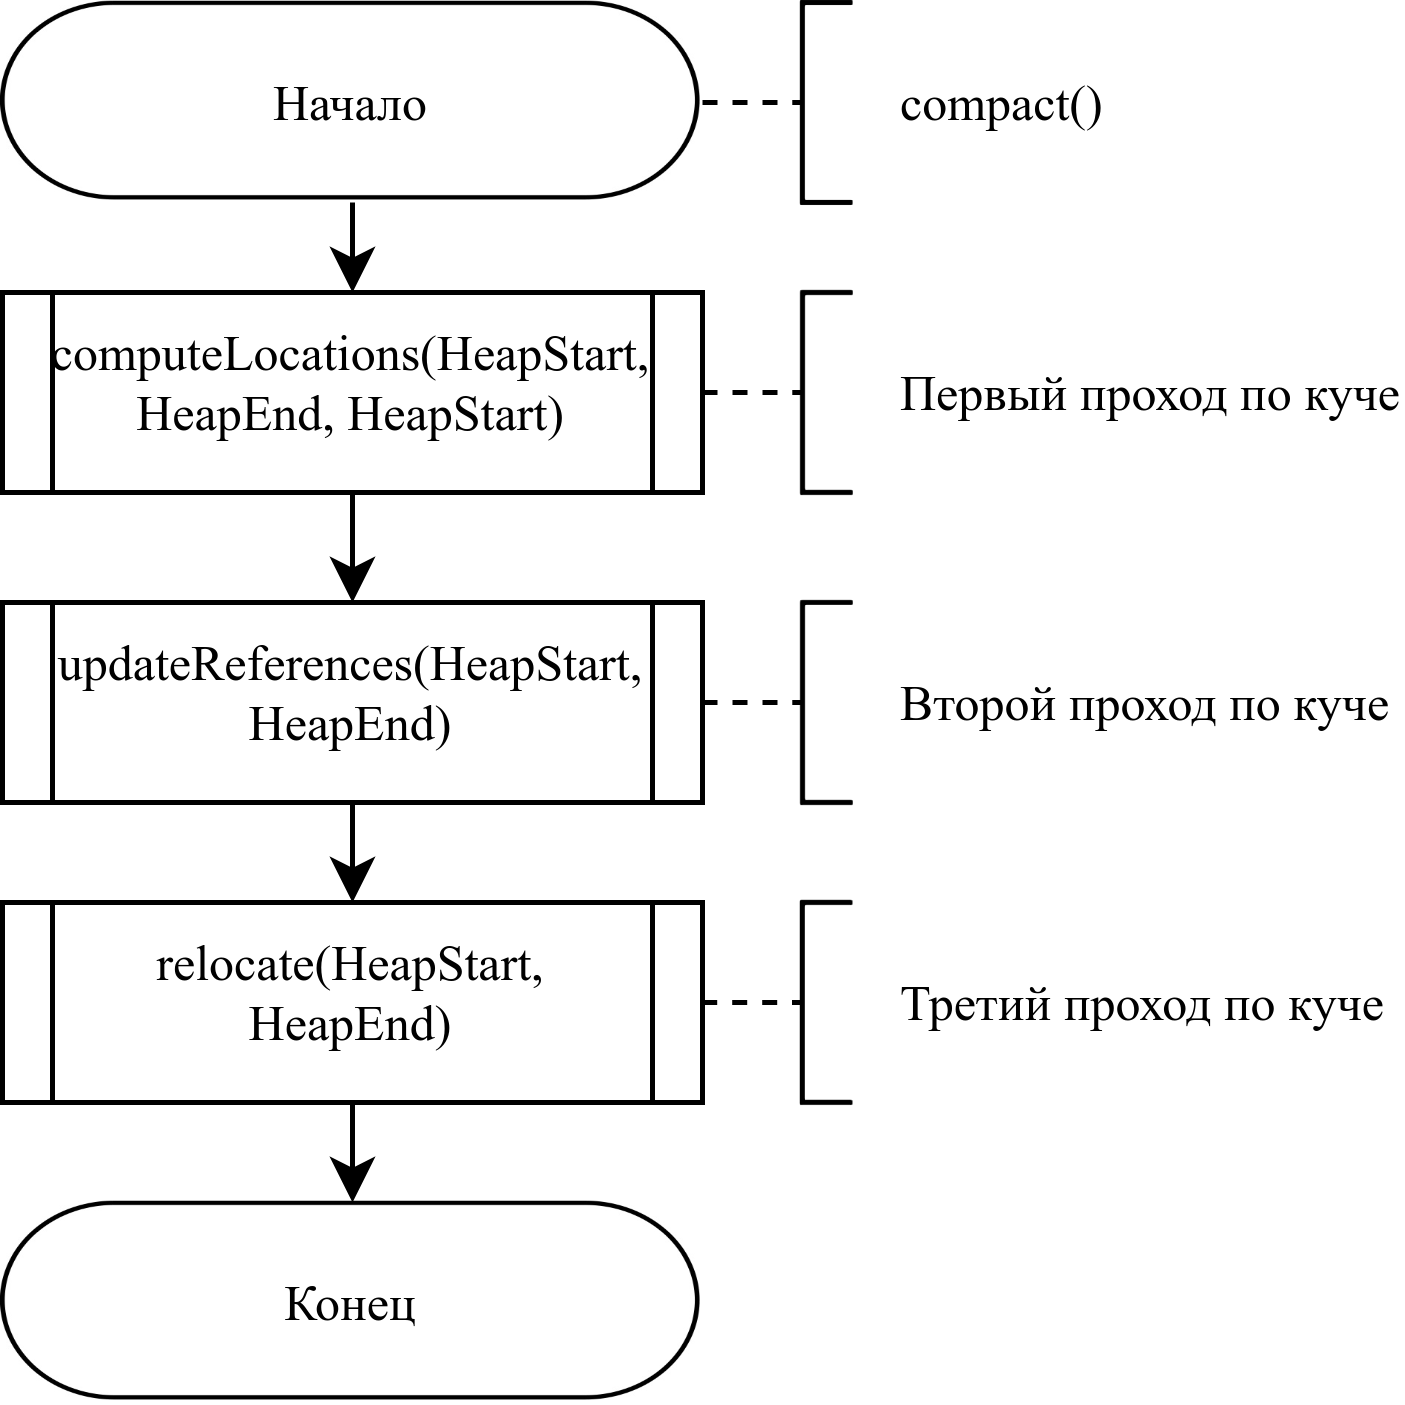
\includegraphics[scale=0.175]{assets/mark-compact-1.png}
	\caption{Функция уплотнения объектов в куче}
	\label{fig:mark-compact-1}
\end{figure}

\begin{figure}[H]
	\centering
	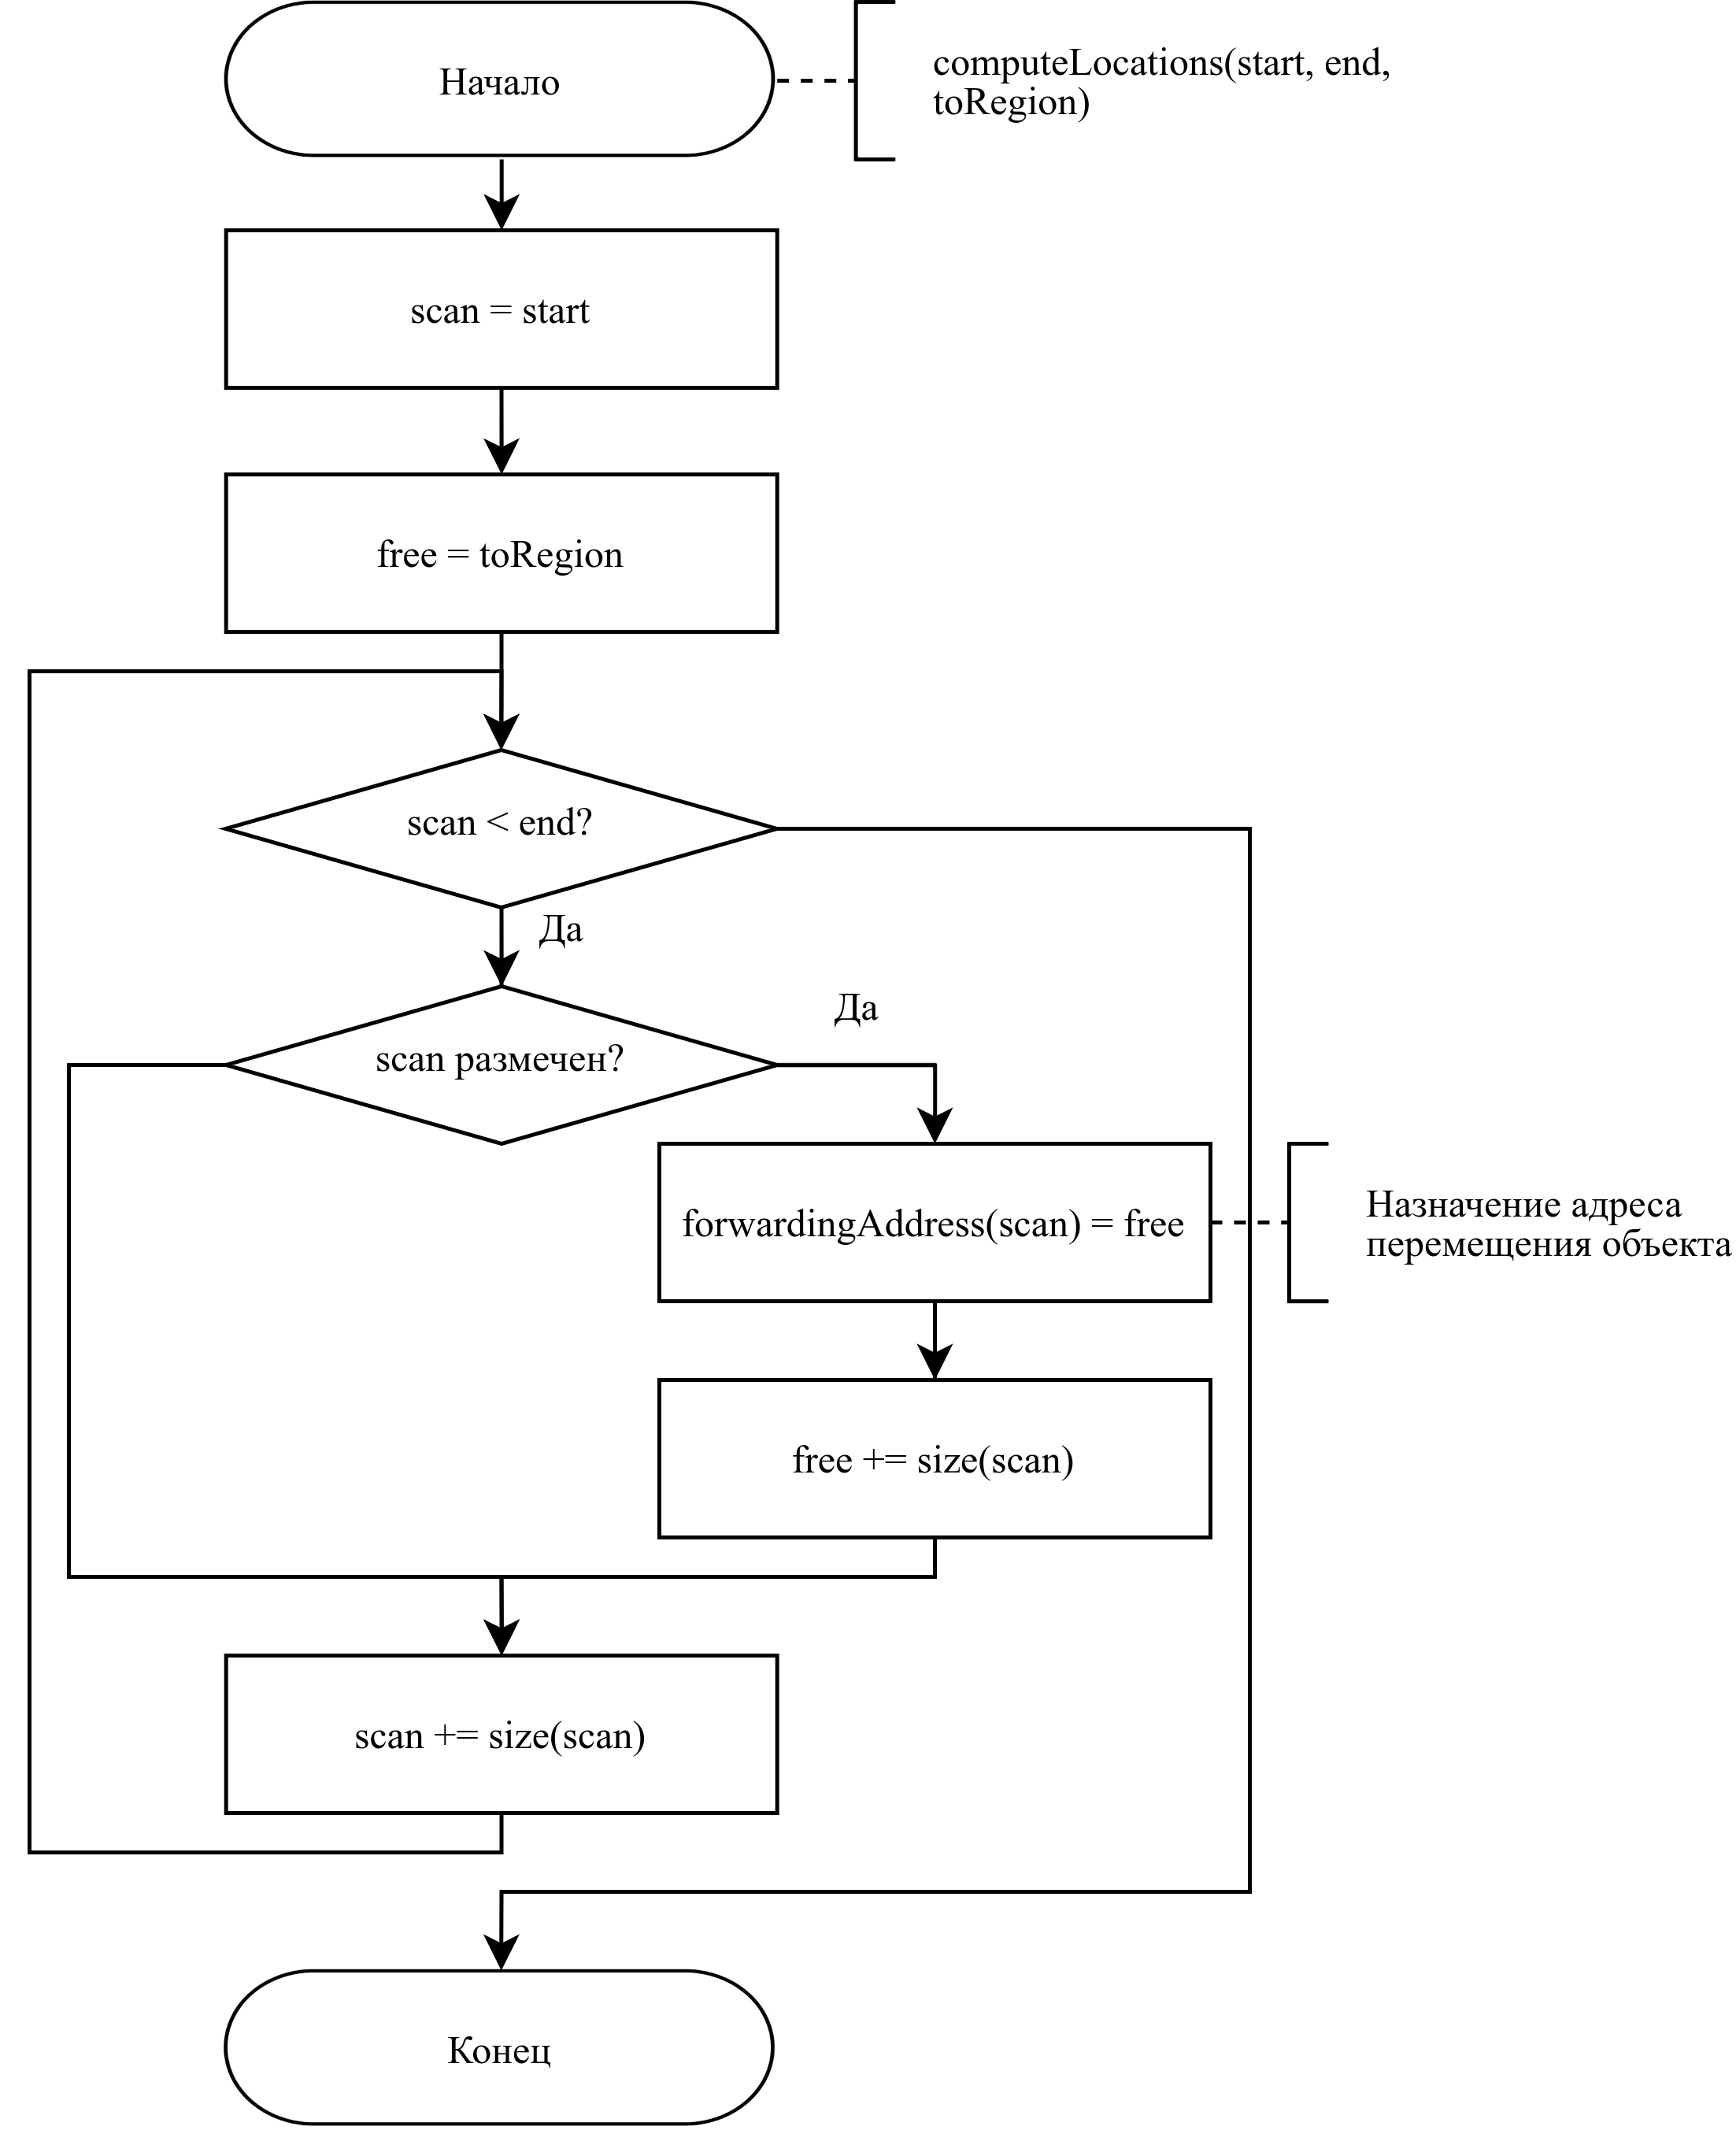
\includegraphics[scale=0.175]{assets/mark-compact-2.png}
	\caption{Первый проход по куче: вычисление адресов перемещения используемых объектов}
	\label{fig:mark-compact-2}
\end{figure}

\begin{figure}[H]
	\centering
	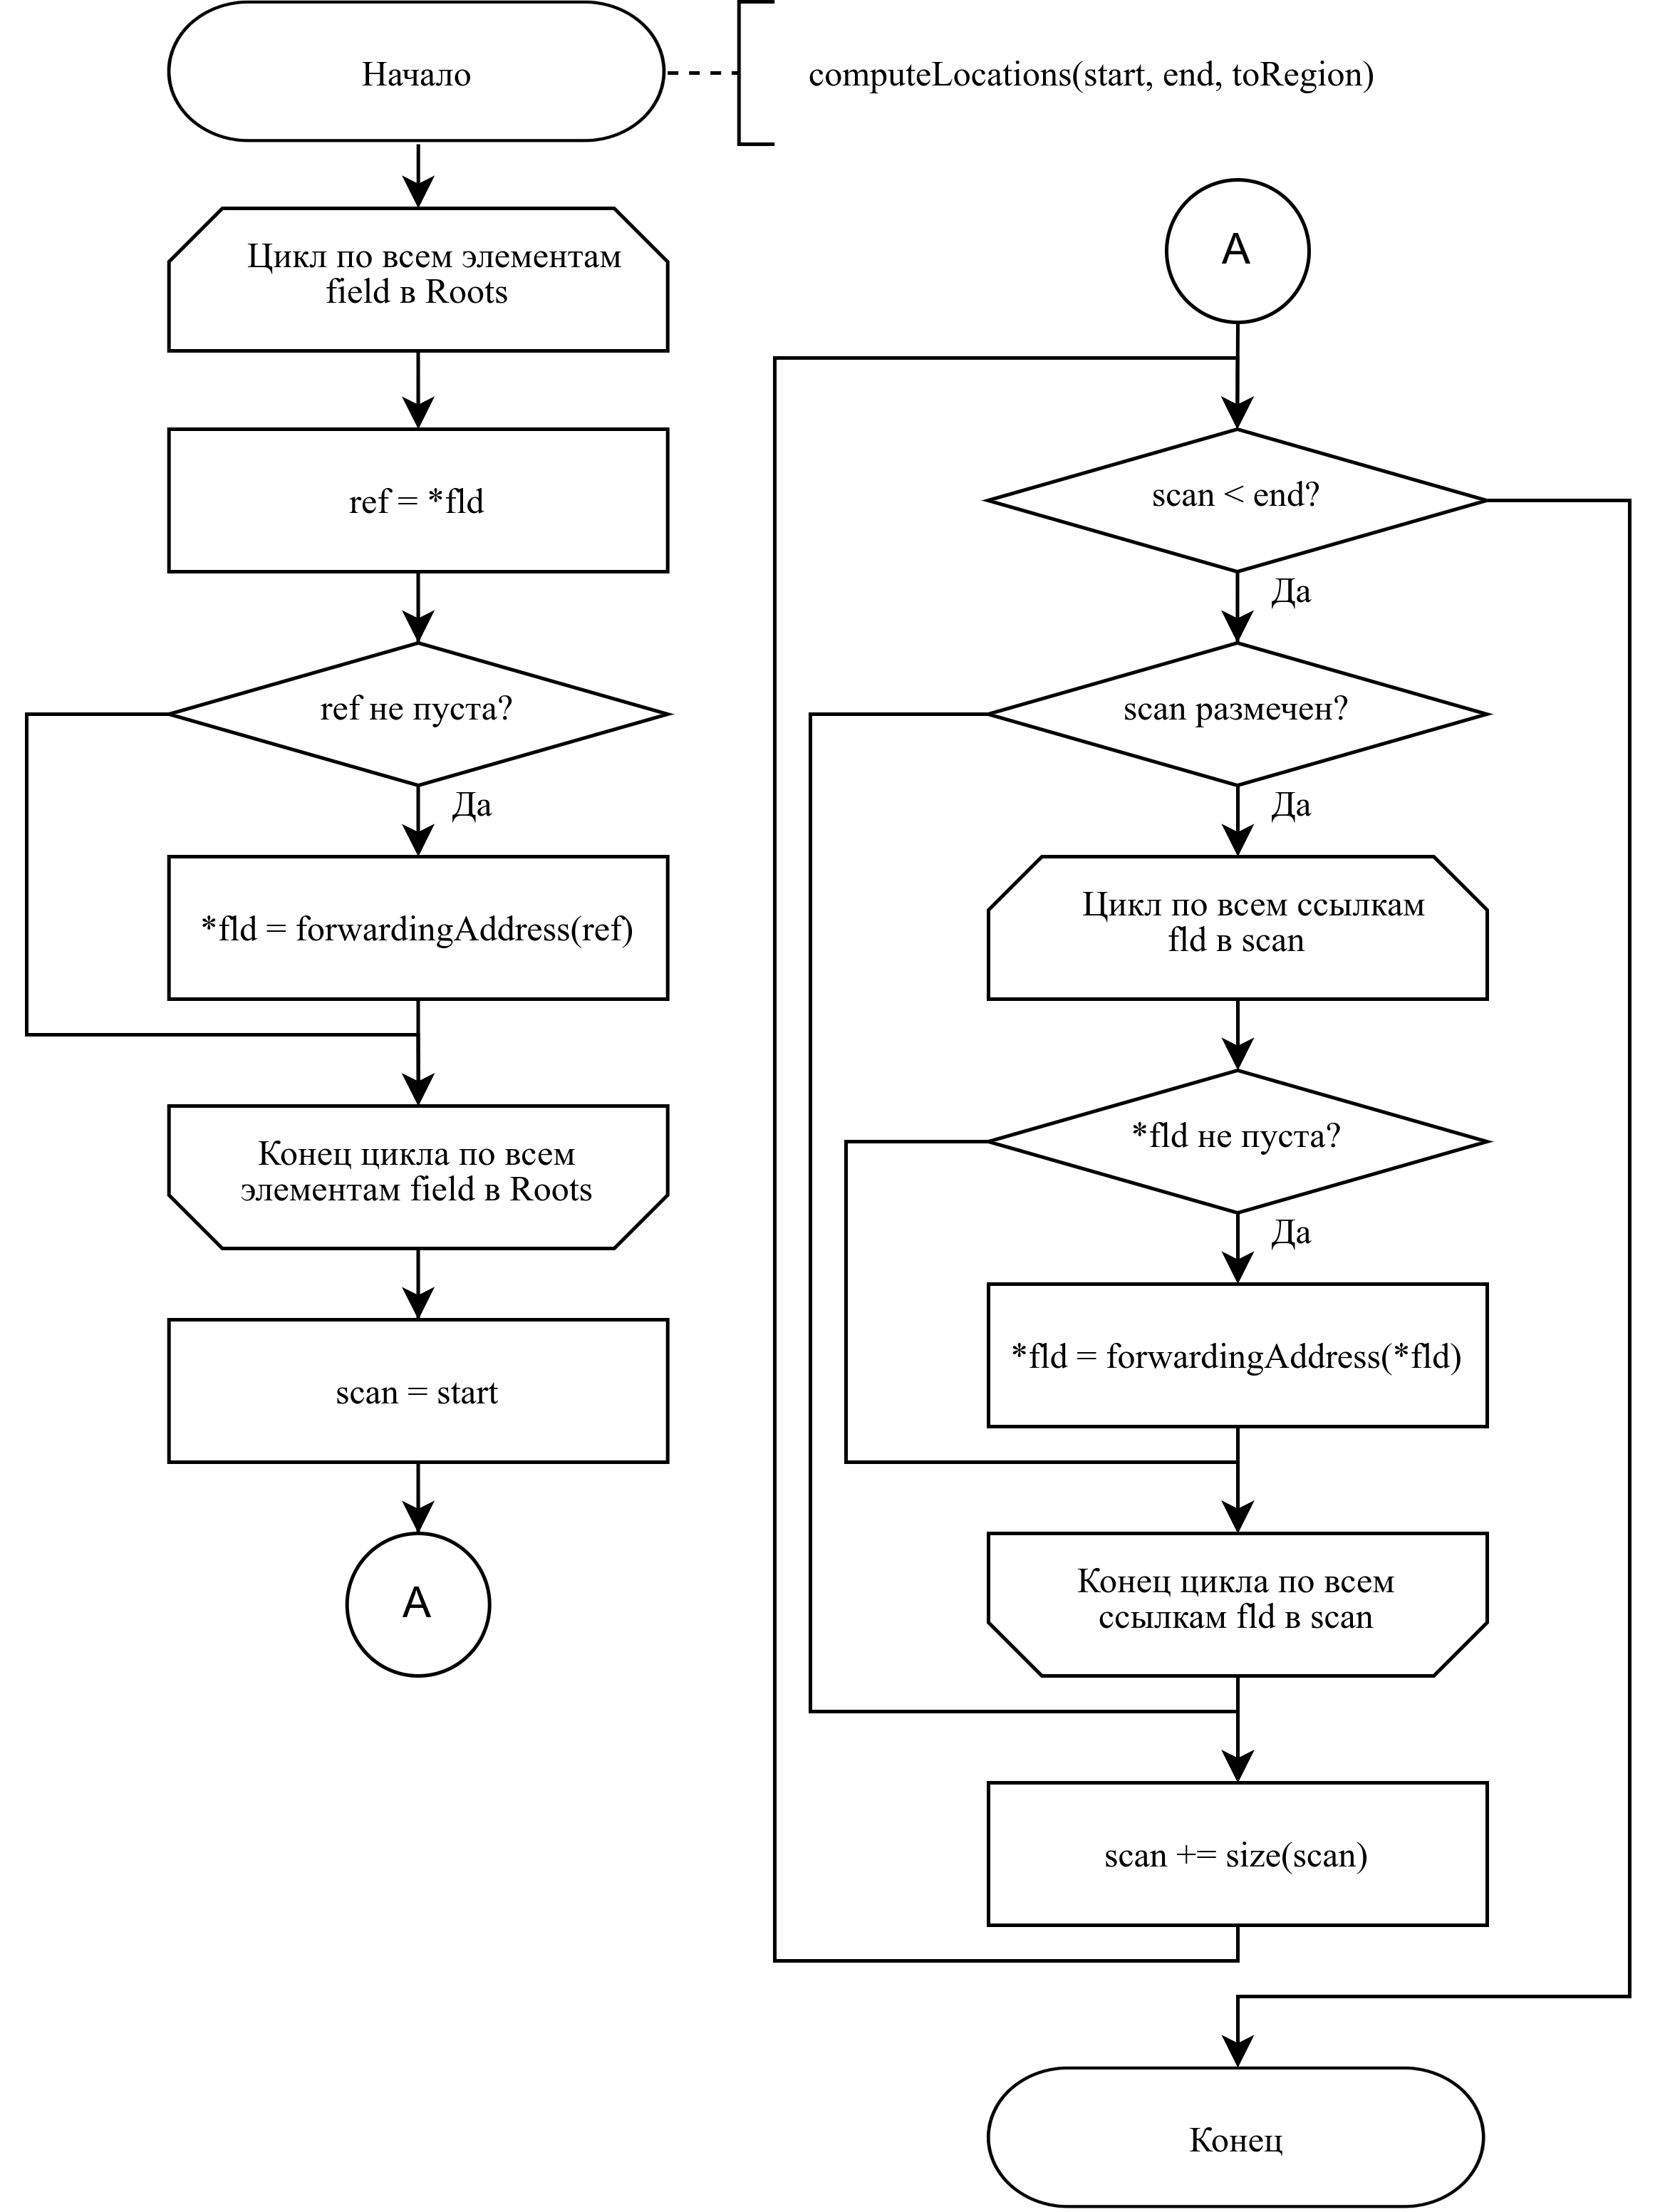
\includegraphics[scale=0.175]{assets/mark-compact-3.png}
	\caption{Второй проход по куче: обновление ссылок в корневом наборе и в размеченных объектах}
	\label{fig:mark-compact-3}
\end{figure}

\begin{figure}[H]
	\centering
	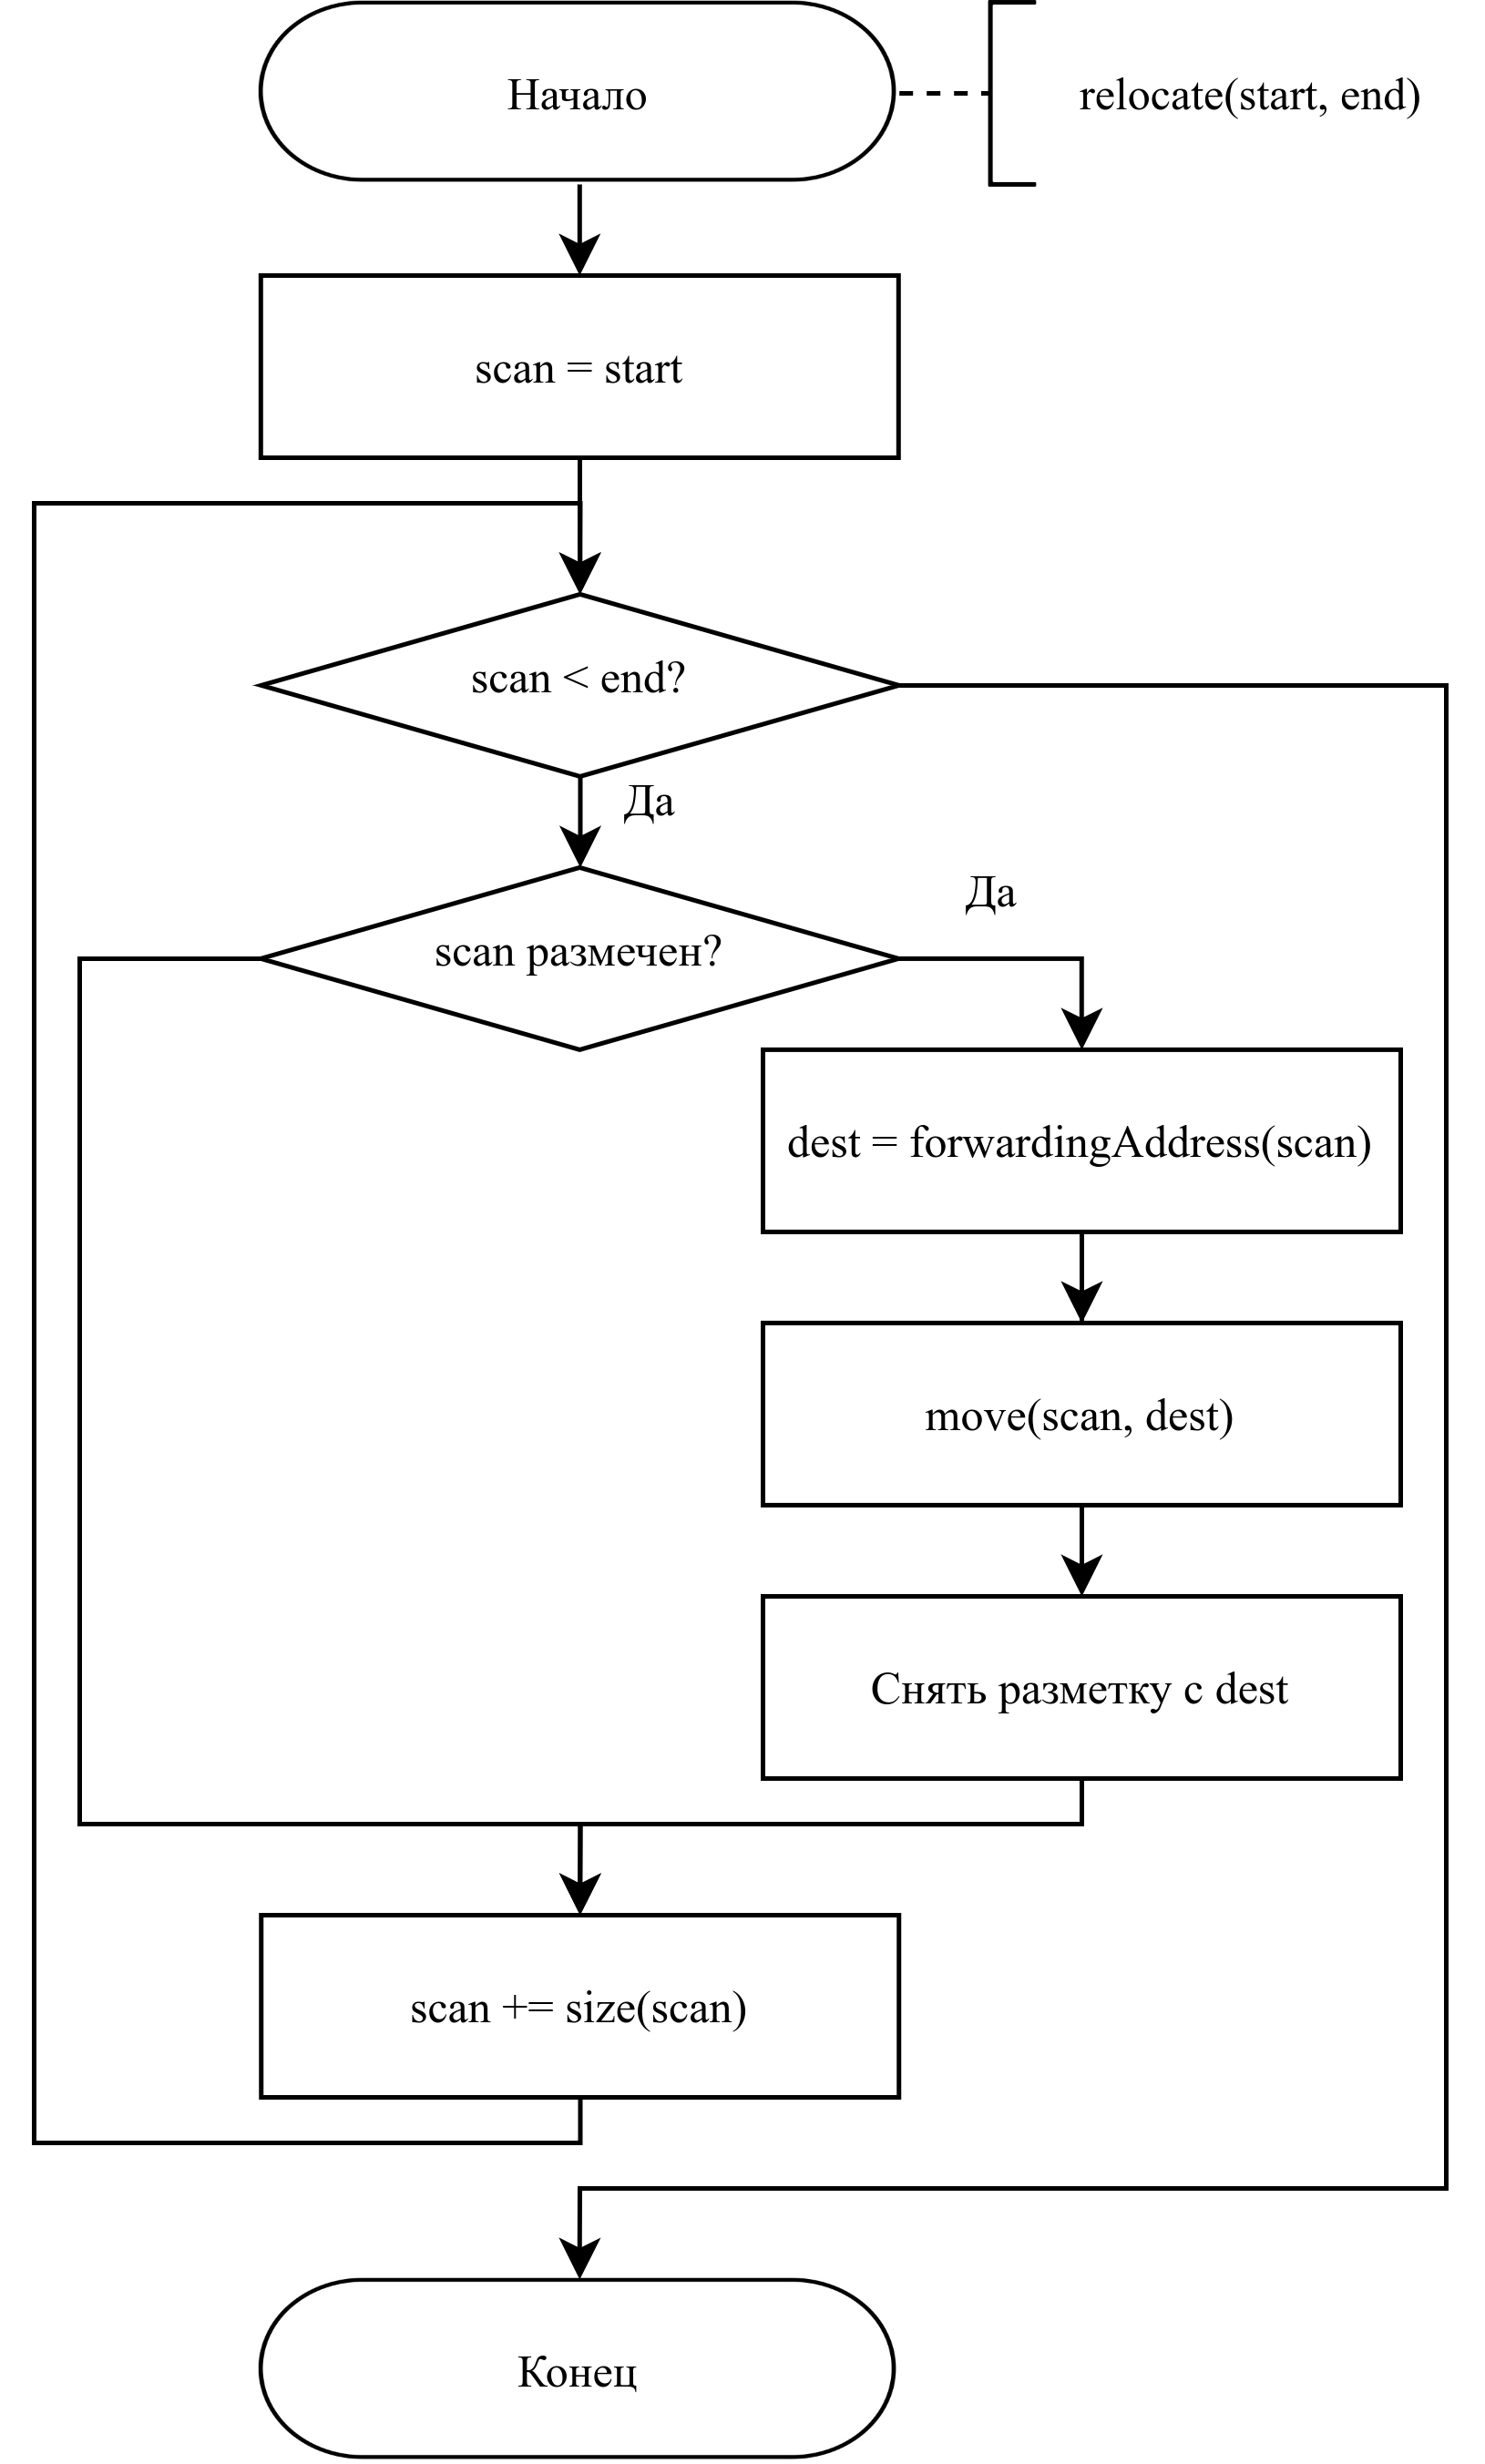
\includegraphics[scale=0.175]{assets/mark-compact-4.png}
	\caption{Третий проход по куче: перемещение используемых объектов}
	\label{fig:mark-compact-4}
\end{figure}

Для сокращения количества проходов сборщика мусора по куче до двух (один для разметки и один для перемещения объектов) и снижения накладных расходов при многопоточной сборке можно хранить адреса перемещения в дополнительной таблице, которая сохраняется во время уплотнения. Данный подход реализуют \textbf{однопроходные алгоритмы}.

%Если мы хотим сократить количество проходов скользящего сборщика по куче до двух
%(один для пометки и один для перемещения объектов) и избежать затрат на многопоточность, то мы должны
%хранить адреса пересылки в дополнительной таблице, которая сохраняется во время сжатия. Абуа-
%Иадх и др. [2004], а также Кермани и Петранк [2006] разработали высокопроизводительные алгоритмы mark-
%compact для мультипроцессоров, которые делают именно это. Первый представляет собой параллельный
%алгоритм остановки мира (он использует несколько потоков сжатия); второй может быть can
%также может быть сконфигурирован как параллельный (позволяющий потокам-мутаторам запускаться параллельно
%потокам-коллекторам) и инкрементный (периодически ненадолго приостанавливающий поток-мутатор для выполнения
%небольшого объема работы по уплотнению). Мы обсудим параллельные, параллелепипедические и
%инкрементальные аспекты этих алгоритмов в последующих главах. Здесь мы сосредоточимся на основных
%алгоритмах сжатия в условиях "остановки мира".
%Оба алгоритма используют несколько дополнительных таблиц или векторов. Обычная для многих коллекционеров
%маркировка использует растровое изображение с одним битом для каждой гранулы (скажем, слова). Маркировка устанавливает биты
%соответствует первой и последней гранулам каждого живого объекта. Например, биты 16 и
%19 установлены для объекта, помеченного как старый на рис. 3.3. Внимательно изучая растровое изображение метки на этапе
%уплотнения, сборщик может рассчитать размер любого живого объекта.
%
%Во-вторых, таблица используется для хранения адресов пересылки. Было бы непомерно
%дорого делать это для каждого объекта (особенно если мы предполагаем, что объекты выровнены по словам), поэтому
%оба этих алгоритма делят кучу на небольшие блоки одинакового размера (256 или 512
%байт соответственно). Таблица смещений хранит адрес пересылки первого живого объекта в каждом
%блоке. Новые местоположения других живых объектов в блоке могут быть вычислены "на лету
%" на основе векторов смещения и меток-битов. Аналогично, учитывая ссылку на любой объект, мы можем
%вычислите номер его блока и, таким образом, выведите его адрес пересылки из записи в таблице
%смещений и битов меток для этого блока. Это позволяет алгоритмам заменять
%многократные проходы по всей куче для перемещения объектов и обновления указателей одним проходом
%по вектору битов меток для построения вектора смещения и одним проходом по куче (после
%разметки) для перемещения объектов и обновления ссылок, сверяясь с этими суммарными векторами.
%Уменьшение количества проходов кучи имеет, как следствие, преимущества для локальности. Давайте рассмотрим
%детали в том виде, в каком они представлены в алгоритме 3.4.
%После завершения разметки процедура
%computeLocations обрабатывает вектор битов меток для получения вектора смещения. По сути, он выполняет те же вычисления, что и в
%Lisp 2 (алгоритм 3.2), но не нужно касаться какого-либо объекта в куче. Например,
%рассмотрим первый отмеченный объект в блоке 2, показанный жирным шрифтом на рисунке 3.3. Биты 2
%и 3, а также 6 и 7 установлены в первом блоке, а биты 3 и 5 - во втором (в этом примере
%каждый блок содержит восемь слотов). Это представляет собой 7 гранул (слов), которые отмечены в
%растровое изображение перед этим объектом. Таким образом, первый живой объект в блоке 2 будет перемещен в
%седьмой слот в куче. Этот адрес записан в векторе смещения для блока (см.
%пунктирную стрелку с пометкой смещение [блок] на рисунке).
%Как только вектор смещения вычислен, корневые и текущие поля обновляются, чтобы
%отразить новые местоположения. Алгоритм Lisp 2 должен был разделять обновление ссылок
%и перемещение объектов, потому что информация о перемещении хранилась в куче, а
%перемещение объекта уничтожало эту информацию, поскольку перемещенные объекты скользили поверх старых объектов. В кон-
%обычно алгоритмы типа Compressor перемещают объекты и обновляют ссылки за один проход,
%updatereferencesrelocate в алгоритме 3.4. Это возможно, потому что новые адреса
%могут быть вычислены достаточно быстро из растрового изображения меток и вектора смещения "на
%лету": компрессору не нужно хранить адреса пересылки в куче. Учитывая
%адрес любого объекта в куче, newAddress получает номер его блока (через shift



\subsubsection{Копирующая сборка мусора}

Третий метод трассирующей сборки мусора --- полупространственное копирование (semispace copying). Уплотнение кучи в данном подходе обеспечивает быстрое распределение и требует только одного прохода по используемым объектам в куче. Его главным недостатком является то, что он уменьшает размер доступной кучи вдвое. \cite{handbook}

Как правило, сборщики копирования делят кучу на два полупространства равного размера, называемых \textbf{старым} (old space, fromspace) и \textbf{новым пространством} (new space, tospace). Создаваемые объекты размещаются в <<новом пространстве>>, если имеется достаточное количество памяти, иначе запускается сборка мусора. На абстрактном уровне всё, что делает копирующий сборщик мусора, --- начинает с корневого набора и обходит все доступные объекты, выделенные в памяти, копируя их из одного полупространства в другое. При копировании объектов происходит их уплотнение таким образом, чтобы они занимали непрерывную область памяти. После копирования объектов <<старое пространство>> освобождается. Такой подход устраняет <<дыры>> в памяти, занимаемые неиспользуемыми объектами. После копирования и уплотнения получается сжатая копия данных в <<новом пространстве>> и, возможно, увеличивается непрерывная область памяти в <<старом пространстве>>, в котором можно размещать новые объекты. На следующем цикле сборки мусора <<старое>> и <<новое>> пространства меняются ролями. \cite{handbook} \cite{cornell3}

На рисунках \ref{fig:copying-1}-\ref{fig:copying-3} представлены схемы алгоритма копирующей сборки мусора, использующего полупространственное копирование. \cite{handbook}

\begin{figure}[H]
	\centering
	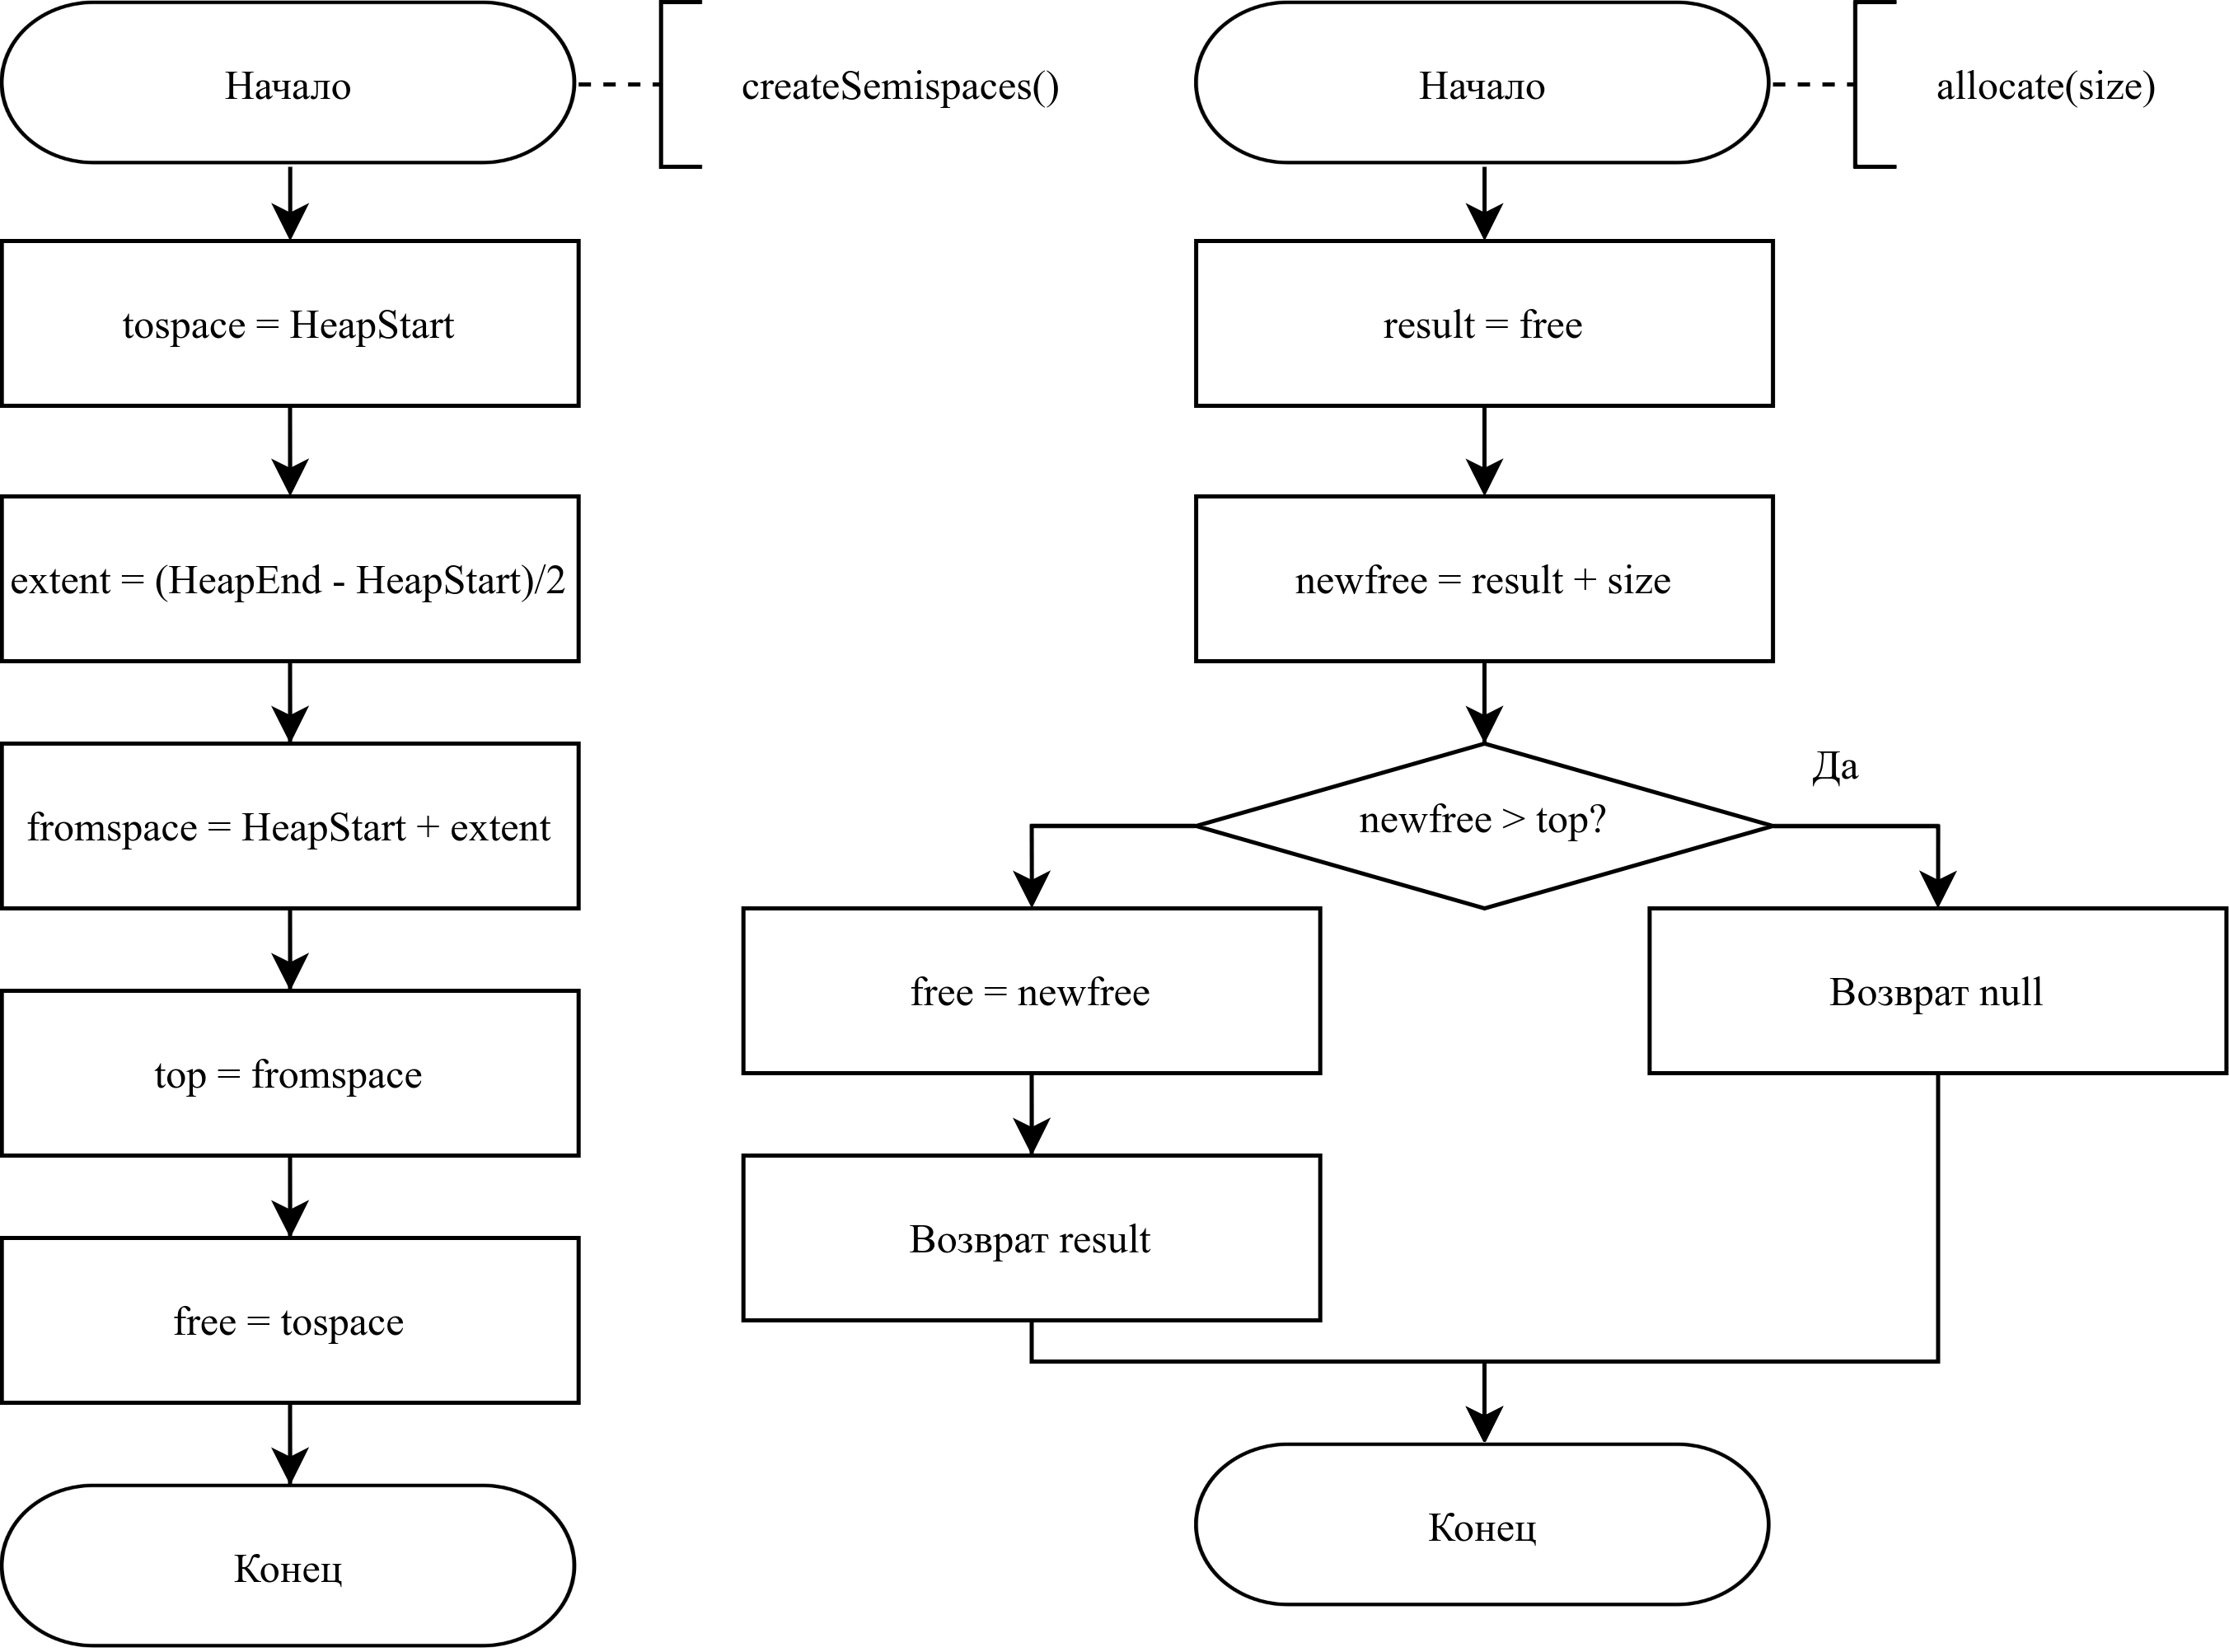
\includegraphics[scale=0.175]{assets/copying-1.png}
	\caption{Функции для создания полупространств кучи и выделения памяти в них}
	\label{fig:copying-1}
\end{figure}

\begin{figure}[H]
	\centering
	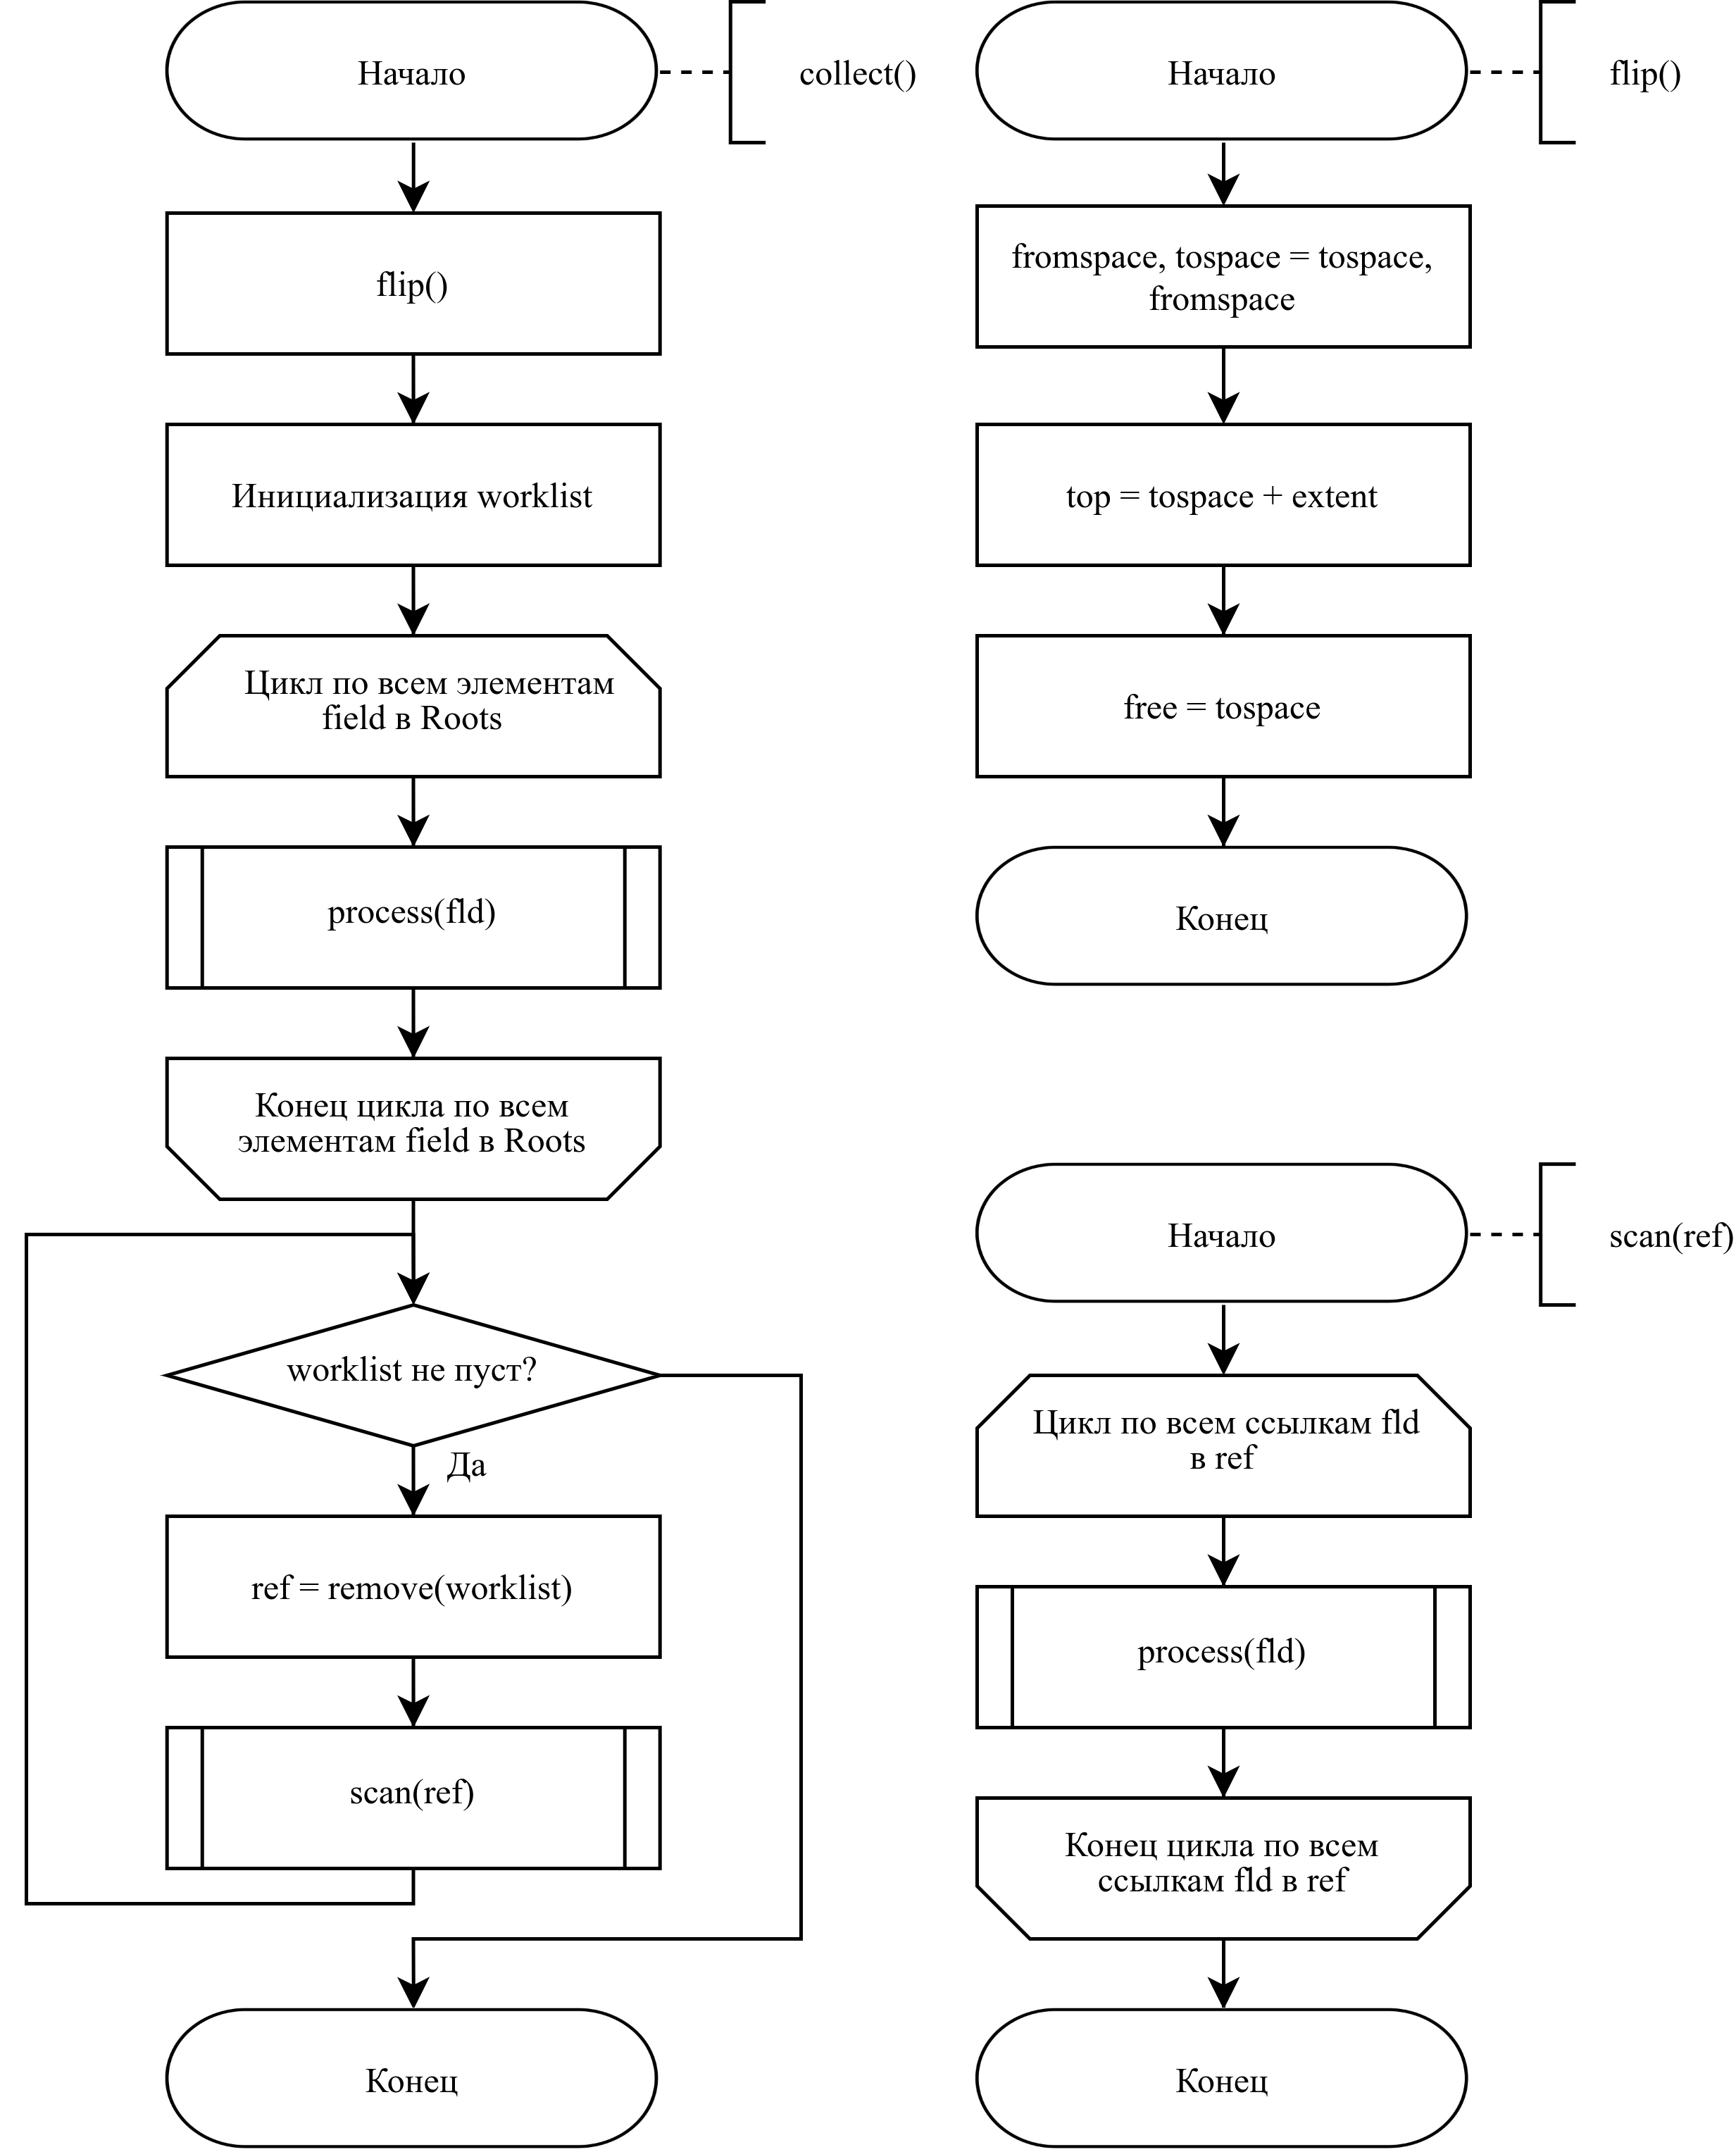
\includegraphics[scale=0.175]{assets/copying-2.png}
	\caption{Функции для сбора мусора, обмена полупространств местами и сканирования ссылки на объект}
	\label{fig:copying-2}
\end{figure}

\begin{figure}[H]
	\centering
	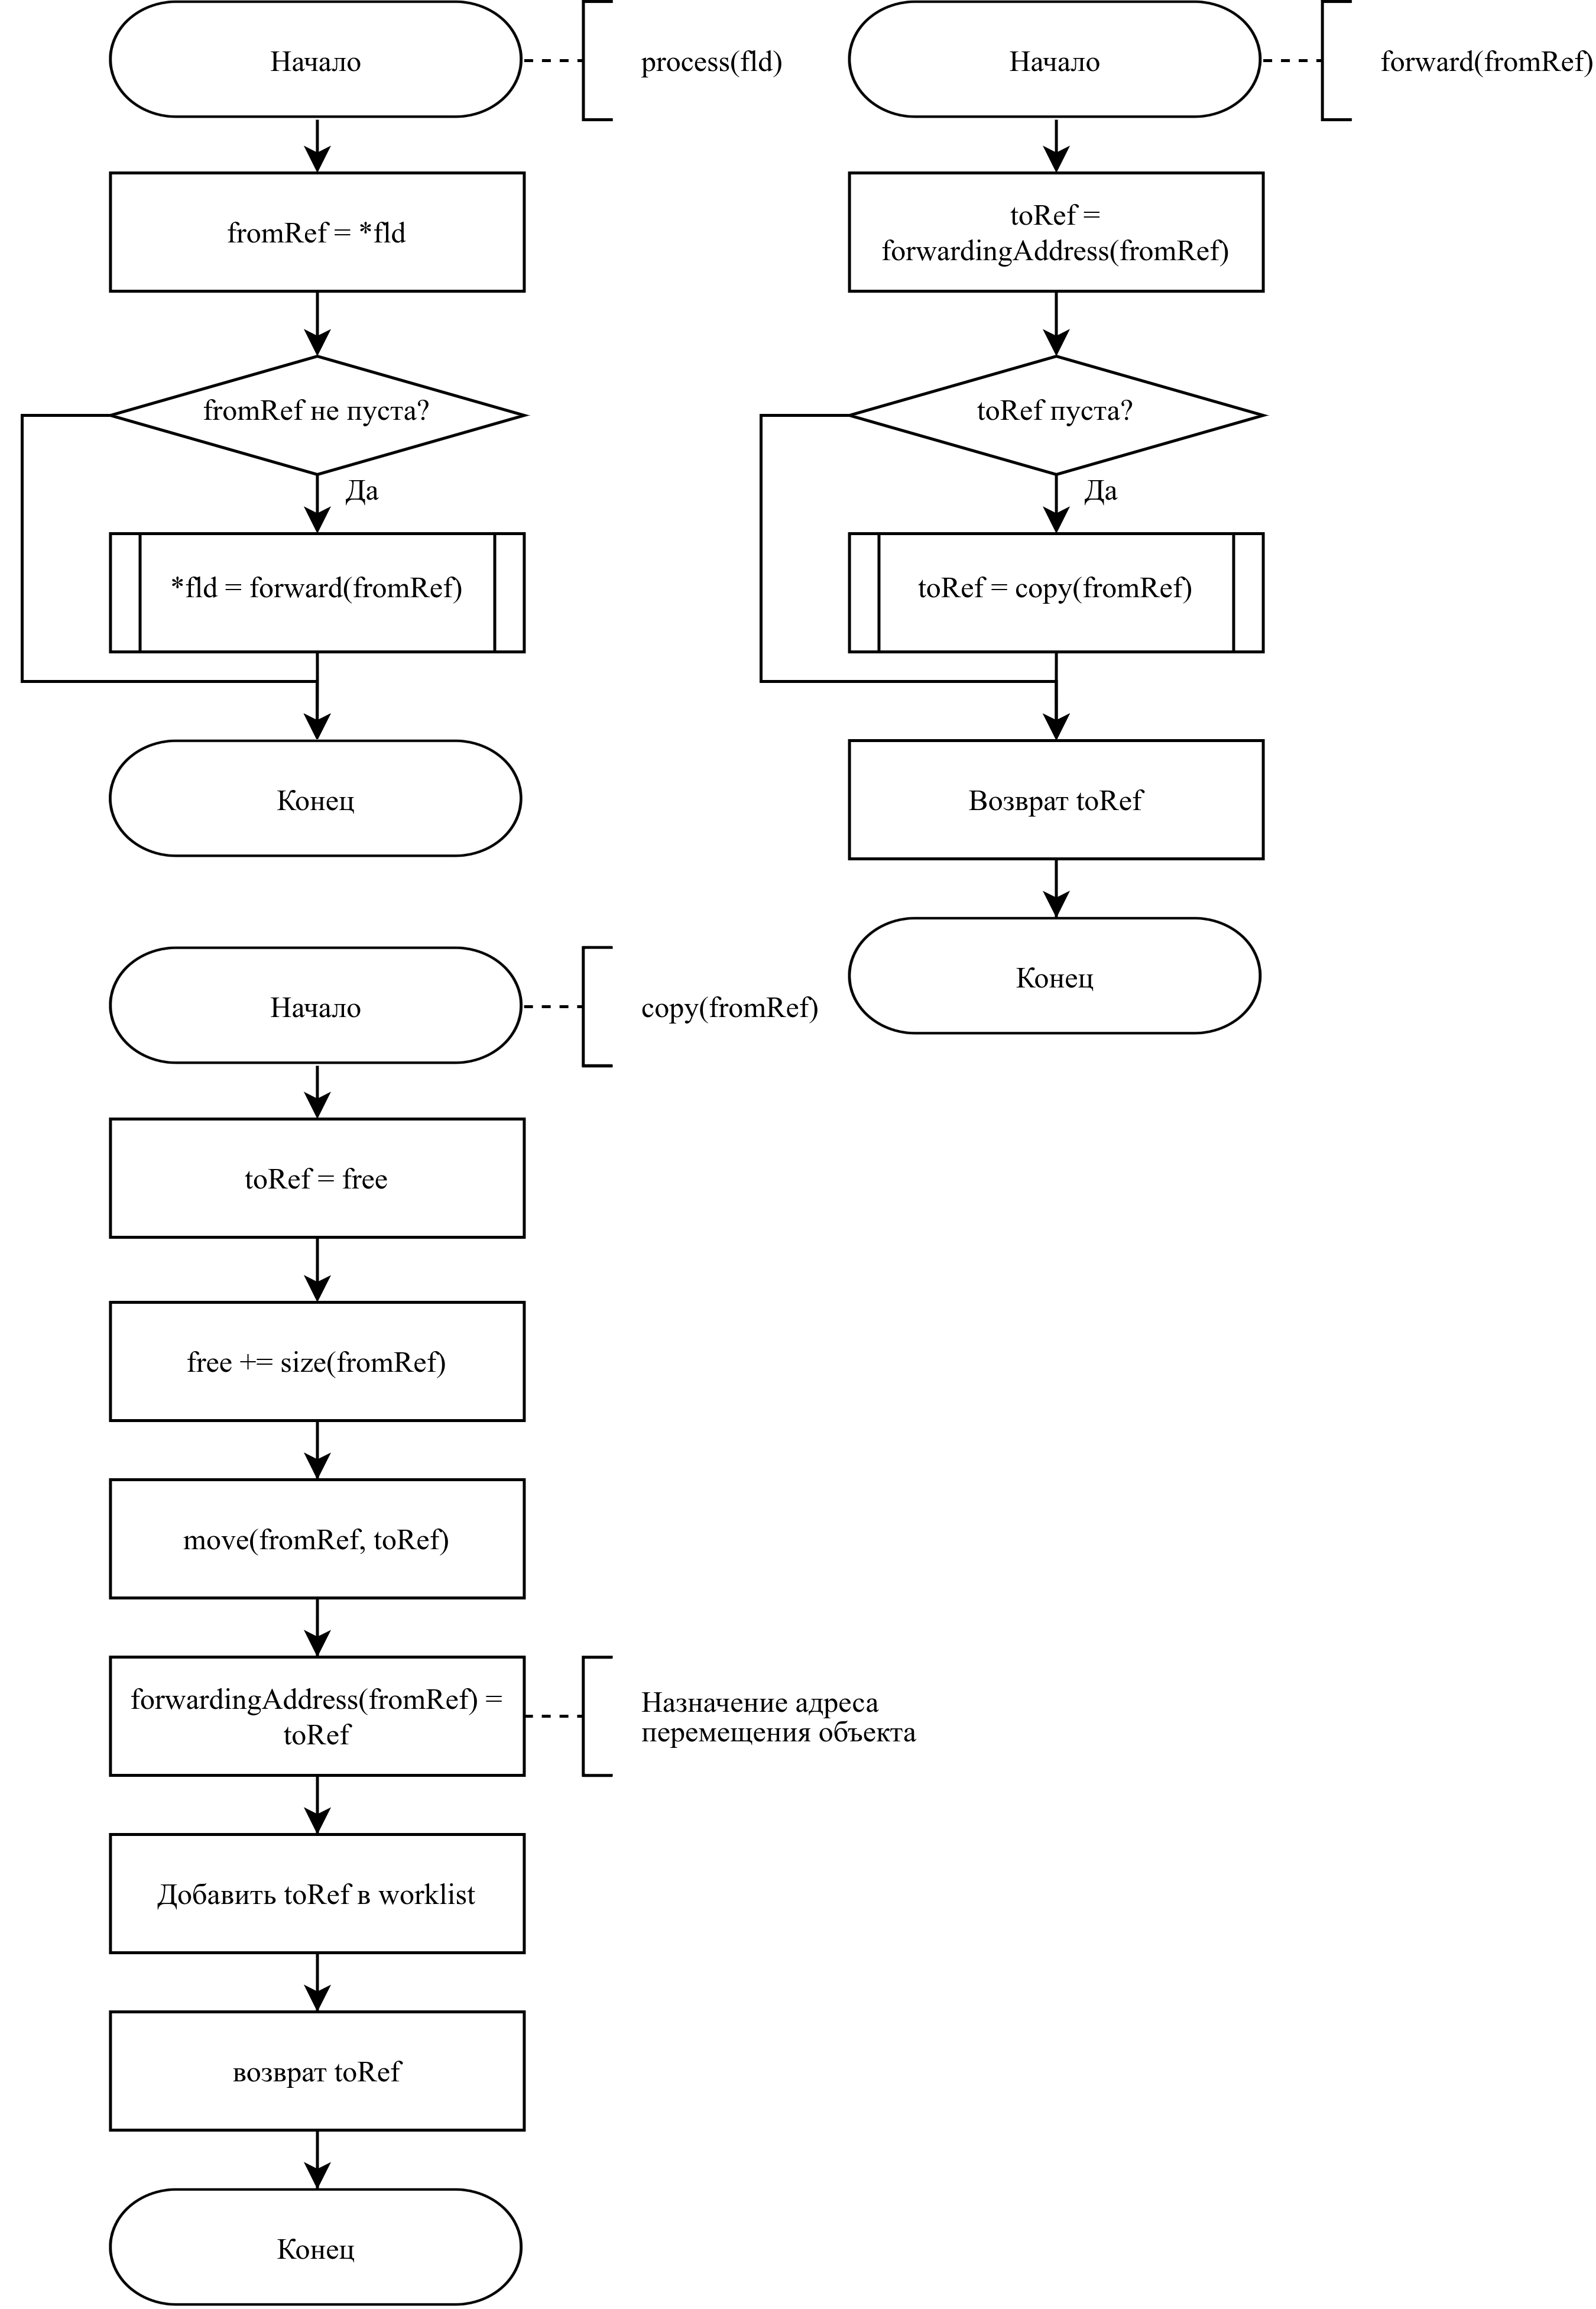
\includegraphics[scale=0.175]{assets/copying-3.png}
	\caption{Функции для перемещения и обновления ссылки на объект}
	\label{fig:copying-3}
\end{figure}

Важным недостатком полупространственного копирования является необходимость хранения второго полупространства, иногда называемого \textbf{резервом копирования} (copy reserve), без возможности выделять память в нём. При ограниченном объёме доступной памяти и игнорировании структур данных, необходимых сборщику мусора, такой подход к распределению памяти обеспечивает возможность работы только с половиной пространства кучи, что существенно меньше того объёма памяти, который предоставляют другие менеджеры памяти. Следовательно, копирующие сборщики мусора будут выполнять больше циклов сборки, чем другие сборщики. Приведёт ли это к изменению производительности, зависит от характеристик прикладной программы и объёма доступного пространства в куче. \cite{handbook}

Анализ асимптотической сложности может свидетельствовать в пользу копирующей сборки мусора. Пусть M --- общий размер кучи, а L --- объём используемых данных. Сборщики полупространств должны копировать, сканировать и обновлять указатели в L. Сборщики, работающие по алгоритму mark-sweep, должны аналогичным образом отслеживать все используемые объекты и затем зачищать всю кучу. Временные сложности алгоритмов mark-sweep и semispace copying можно определить следующим образом: \cite{handbook}

\begin{equation}
	t_{MS} = mL + sM,
\end{equation}

\begin{equation}
	t_{Copy} = cL,
\end{equation}
где c, m и s --- некоторые коэффициенты, не зависящие от M и L.

Объем памяти, освобождаемый каждым сборщиком, равен

\begin{equation}
	m_{MS} = M - L,
\end{equation}

\begin{equation}
	m_{Copy} = M/2 - L.
\end{equation}

Пусть r = L/M --- размер используемых данных в куче, которые мы предполагаем постоянными. Так, эффективность алгоритма может быть описана количеством работы, выполненной сборщиком мусора при выделении одного объекта (соотношение <<mark/cons>> \cite{handbook}).

\begin{equation}
	e_{MS} = \frac{mr + s}{1 - r},
\end{equation}

\begin{equation}
	e_{Copy} = \frac{2cr}{1 - 2r}.
\end{equation}

На рисунке \ref{fig:complexity} представлен график зависимости эффективности алгоритма сборки мусора (e) от доли используемых объектов кучи (live ratio). \cite{handbook}

\begin{figure}[H]
	\centering
	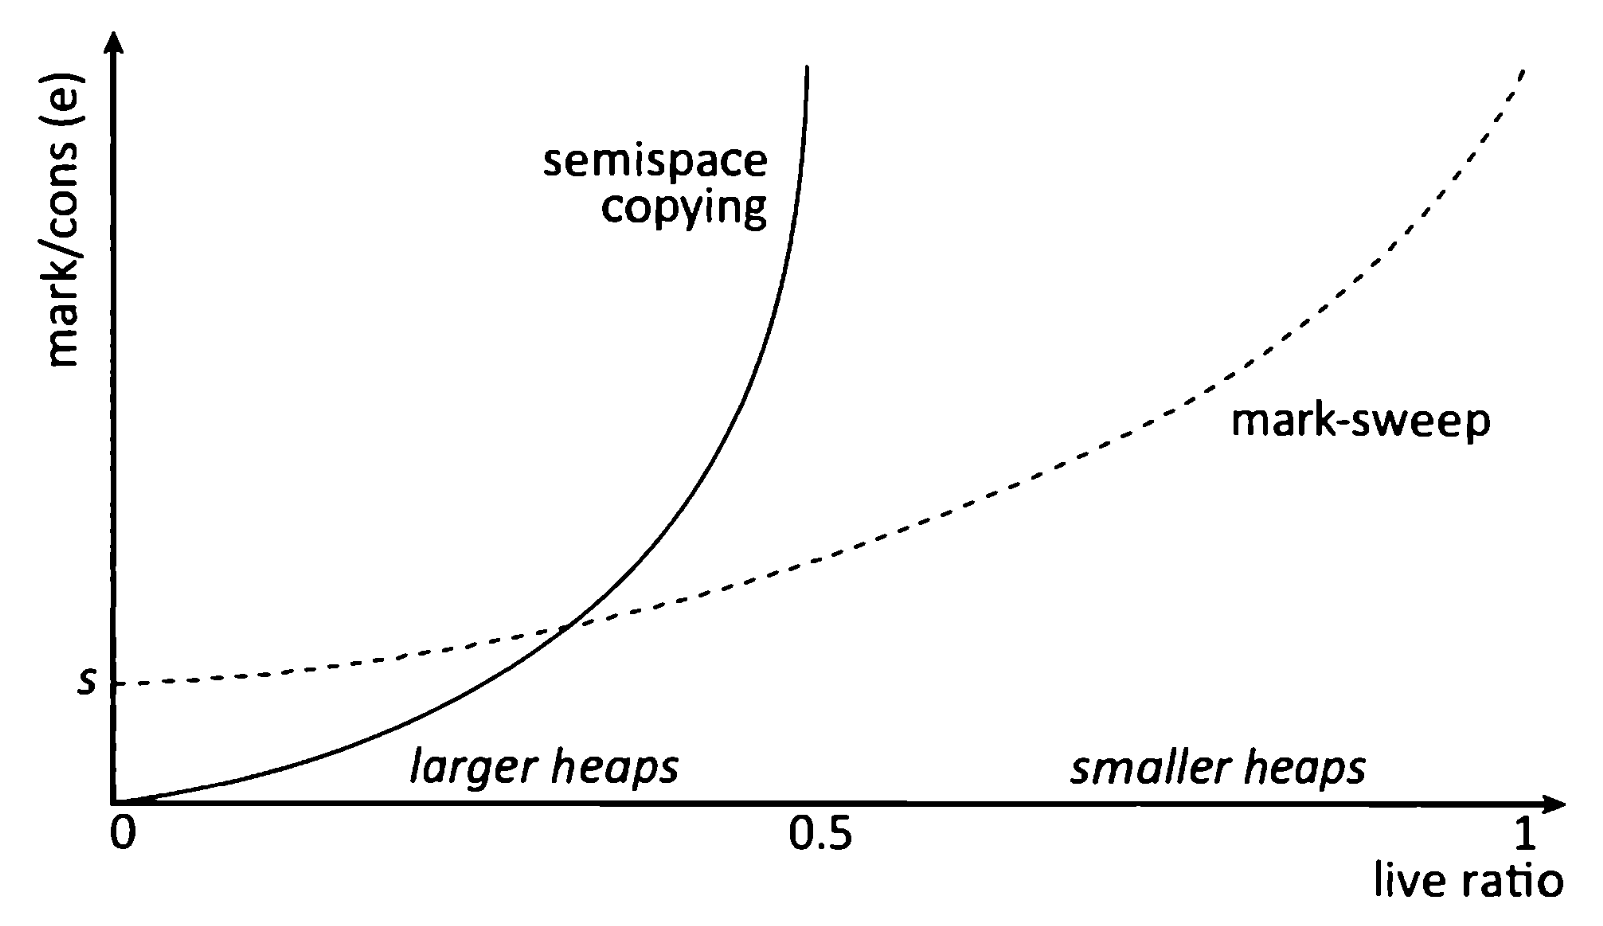
\includegraphics[width=\textwidth]{assets/complexity.png}
	\caption{Соотношение <<mark/cons>> для алгоритмов mark-sweep и semispace copying (чем меньше, тем алгоритм эффективнее)}
	\label{fig:complexity}
\end{figure}

Как показал анализ асимптотической сложности, алгоритм semispace copying может быть более эффективным, чем mark-sweep, при условии, что куча достаточно велика, а коэффициент r достаточно мал. Стоит заметить, что такой анализ игнорирует некоторые аспекты реализации алгоритмов. Современные сборщики, основанные на алгоритме mark-sweep, зачастую используют \textbf{ленивую зачистку} (lazy sweep, очистка памяти при выделении), тем самым уменьшая константу s и снижая соотношение e. Также анализ сложности игнорирует преимущество локализации объектов при последовательном распределении, когда объекты, к которым доступ осуществляется одновременно, размещаются в соседних областях памяти (см. п. \ref{memory_management}).



\subsubsection{Алгоритм поколений}
\label{generational}

Одна из основных проблем копирующего сборщика мусора заключается в том, что ему приходится просматривать всю кучу при каждом запуске сборки мусора. Объекты в памяти обладают важным свойством временной устойчивости, которое можно сформулировать в виде следующей гипотезы. \cite{cornell3}

\textbf{Гипотеза поколений} (generational hypothesis, infant mortality) \cite{glossary} --- это наблюдение, согласно которому в большинстве случаев <<молодые>> объекты (те, которые создаются позже), с гораздо большей вероятностью перестают использоваться (<<умирают>>) раньше, чем <<старые>> объекты. Строго говоря, гипотеза состоит в том, что вероятность смерти объекта как функция его возраста (времени жизни) убывает гиперэкспоненциально.

\textbf{Сборка мусора по алгоритму поколений} \cite{glossary} --- это трассирующая сборка мусора, в которой используется гипотеза поколений. \textbf{Поколением} называется группа объектов со схожим временем жизни. Новые объекты выделяются в самом молодом поколении и передаются в старшие поколения, если они выживают. Объекты более старых поколений обрабатываются реже, что экономит время процессора.

Как правило, объекты одного поколения имеют мало ссылок на объекты более молодых поколений. Это означает, что сканирование старых поколений в процессе сбора более молодых поколений можно осуществлять реже, отдельно запоминая ссылки на объекты более молодых поколений. \cite{cornell3}

% В широком смысле, поколение объектов --- это набор объектов, которые имеют схожее время жизни.

Использование гипотезы поколений позволяет модифицировать алгоритм копирующей сборки мусора. Так, первоначально созданные объекты будут размещены в области памяти, называемой первым поколением. Когда оно заполняется, производится копирование используемых объектов в другую область памяти, называемую вторым поколением, и освобождается первое поколение. Такая последовательность действий повторяется для новых поколений. \cite{cornell3}



\subsection{Подсчёт ссылок}

Подсчёт ссылок предполагает отслеживание количества указателей на определённые области памяти из других областей. Он используется в качестве основы для некоторых методов автоматической переработки, которые не требуют отслеживания (трассировки). \cite{recycling}

Системы подсчёта ссылок выполняют автоматическое управление памятью, сохраняя в каждом объекте, обычно в заголовке, число ссылок на данный объект. Объекты, на которые нет ссылок (счётчик ссылок равен нулю), не могут быть доступны вызывающей стороне. Следовательно, они не используются и могут быть переработаны. \cite{glossary}

Преимущества подсчёта ссылок:

\begin{itemize}[label*=---]
	\item накладные расходы по управлению памятью распределяются по всему времени работы программы; \cite{handbook}
	\item устойчивость к высоким нагрузкам, так как потенциально подсчёт ссылок может переработать объект как только он перестаёт использоваться; \cite{handbook}
	\item масштабируемость по объёму кучи, так как накладные расходы, как правило, зависят только от количества выполняемых операций с указателями на объекты, а не от объема хранимых данных; \cite{handbook}
	\item может быть реализован без помощи среды выполнения языка и без её ведома. \cite{handbook}
\end{itemize}

Недостатки подсчёта ссылок:

\begin{itemize}[label*=---]
	\item требуются накладные расходы на операции чтения и записи для управления числом ссылок;
	\item операции с числом ссылок на объекты должны быть атомарными; \cite{handbook}
	\item случай циклических ссылок требует отдельного рассмотрения; \cite{handbook}
	\item подсчёт ссылок может вызывать паузы, например при освобождении ссылочных структур данных. \cite{handbook}
\end{itemize}

По сравнению со сборкой мусора алгоритмы управления памятью, основанные на подсчёте ссылок, отличаются детерминированностью, предсказуемостью и меньшей вычислительной сложностью. \cite{cornell2} % классно в конце перефразировал слово "простота", я знаю

Подсчёт ссылок наиболее полезен в ситуациях, когда можно гарантировать отсутствие циклических ссылок и сравнительно редкие модификации ссылочных структур данных. Такие условия могут иметь место в некоторых типах структур баз данных и некоторых файловых системах. Подсчёт ссылок также может быть полезен, если важно, чтобы объекты утилизировались своевременно, например, в системах с жёсткими ограничениями памяти. \cite{recycling}

Далее будут подробно описаны некоторые подходы к реализации подсчёта ссылок. \cite{recycling}



\subsubsection{Отложенный подсчёт ссылок}

Отложенный подсчёт ссылок позволяет уменьшить накладные расходы на поддержание счётчика ссылок в актуальном состоянии за счёт отсутствия корректировок при сохранении ссылки в стеке. \cite{glossary}

Как правило, большинство сохранений ссылок производится в локальные переменные, которые хранятся в стеке. Отложенный подсчёт ссылок позволяет обойтись без них и считать только ссылки, хранящиеся в объектах кучи. Это требует поддержки компилятора, но может привести к значительному повышению производительности сборки мусора. \cite{glossary}

Объекты не могут быть возвращены, как только счетчик ссылок на них станет равным нулю, поскольку на них еще могут быть ссылки из переменных на стеке. Такие объекты добавляются в <<таблицу нулевого счёта>> (Zero Count Table, ZCT). Если в куче сохраняется ссылка на объект с нулевым счётчиком, то этот объект удаляется из ZCT. Периодически производится сканирование стека, и все объекты в ZCT, на которые не было ссылок из стека, освобождаются. \cite{glossary}

Стоит заметить, что отложенный подсчёт ссылок не позволяет корректно обрабатывать объекты с циклическими ссылками, поэтому его часто используют вместе с трассирующим сборщиком мусора. \cite{recycling}

\subsubsection{Взвешенный подсчёт ссылок}

Распределенная сборка мусора \cite{glossary} --- это сборка мусора в системе, в которой объекты могут храниться в разных адресных пространствах или на разных машинах. 

Распределенная сборка мусора влечёт за собой накладные расходы на синхронизацию и связь между процессами. Эти расходы особенно высоки при использовании трассирующего сборщика мусора, поэтому вместо него обычно используются другие методы, например взвешенный подсчёт ссылок. \cite{glossary}

Взвешенный подсчёт ссылок \cite{glossary} -- техника подсчёта ссылок, которая широко используется для распределенной сборки мусора из-за низкого уровня межпроцессного взаимодействия.

Межпроцессные ссылки на объекты подсчитываются, но вместо простого подсчёта количества ссылок каждой ссылке присваивается некоторый вес. При создании объекта начальному указателю на него присваивается вес, который, как правило, кратен двум. В объекте записывается сумма весов всех его ссылок. При копировании ссылки её вес делится поровну между новой и оригинальной ссылками. Так как при этой операции сохраняется взвешенная сумма ссылок, то связь с объектом в этот момент не требуется. При удалении ссылки взвешенная сумма ссылки уменьшается на ее вес. Об этом сообщается объекту путем посылки сообщения. Когда счётчик ссылок объекта становится равным нулю, он может быть освобождён. Алгоритм устойчив к протоколам связи, не гарантирующим порядок поступления сообщений об удалении. \cite{glossary}

\subsubsection{Использование счётчика ссылок с ограниченным полем}

При данном подходе к подсчёту ссылок поле, используемое для хранения числа ссылок на объект, имеет ограниченный размер. В частности, число ссылок на объект может быть настолько большим, что не может быть сохранено в этом поле. \cite{glossary}

Исходя из того, что на большинство объектов, как правило, не ссылаются большое количество раз, некоторые системы, использующие подсчёт ссылок, хранят точное количество ссылок только до определенного максимального значения. Если объект имеет больше ссылок, чем это значение, то счетчик фиксируется на максимальном значении и никогда не декрементируется. Предполагается, что такие объекты встречаются редко, но их память никогда не может быть освобождена с помощью подсчёта ссылок. Для освобождения такой памяти часто используется отдельный трассирующий сборщик мусора. \cite{glossary}

\subsubsection{Подсчёт ссылок с флагом}

Подсчёт ссылок с флагом (one-bit reference counting) \cite{glossary} --- это эвристический механизм, позволяющий с минимальными накладными расходами памяти проверить, используется ли объект в программе.

Однобитовый счетчик ссылок является частным случаем счетчика ссылок с ограниченным полем (limited-field reference count). Один бит в объекте, называемый MRB (Multiple Reference Bit), очищается при выделении объекта. Всякий раз, когда создаётся новая ссылка на объект, этот бит устанавливается. Таким образом, MRB=0 означает, что на объект имеется ровно одна ссылка, а MRB=1 --- что на объект может быть более одной ссылки. \cite{glossary}

MRB может храниться в ссылке, а не в объекте. Это уменьшает количество обращений к памяти, связанных с проверкой и установкой MRB. При копировании ссылки устанавливается MRB так же копируется. Если MRB оригинальной ссылки равен 0, то его также необходимо установить. Установка MRB оригинальной ссылки требует, что её местоположение известно и на момент установки не было перезаписано другими данными. \cite{glossary}

Подсчёт ссылок с флагом может использоваться компиляторами для анализа времени жизни объекта. Когда анализ во время компиляции предсказывает, что конкретный объект может быть освобождён (обычно из-за того, что переменная, ссылающаяся на объект, уничтожена), компилятор может сгенерировать код, который будет проверять MRB объекта во время выполнения. Если MRB равен 0, то объект можно освободить. \cite{glossary}

Использование подсчёта ссылок с флагом имеет свои издержки: MRB занимает дополнительную память и его необходимо устанавливать каждый раз, когда количество ссылок на объект увеличивается. Однако эти накладные расходы меньше, чем при использовании других способов подсчёта ссылок, так как MRB занимает всего один бит и счётчик ссылок не корректируется при уничтожении ссылок на объект. \cite{glossary}

\subsubsection{Подсчёт циклических ссылок}

Поскольку число ссылок на объекты, составляющие циклическую структуру данных, не меньше единицы, подсчёт ссылок сам по себе не может восстановить такие структуры. Однако
такие циклы повсеместно используются в программах, например, при создании многосвязных списков и циклических буферов. \cite{handbook}

Наиболее широко распространенные механизмы обработки циклов посредством подсчёта ссылок используют метод, называемый \textbf{пробным удалением}. Его ключевой особенностью является то, что трассирующему сборщику мусора нет необходимости просматривать весь граф используемых объектов. Вместо этого можно рассматривать только те части графа, в которых удаление указателя могло бы привести к циклу сборки мусора. Стоит заметить, что в любой структуре мусорных указателей все ссылки должны быть связаны с внутренними указателями, то есть с указателями между объектами внутри структуры. Циклы сборки мусора могут возникать только при удалении указателя, в результате которого число ссылок на объект становится равным нулю. \cite{handbook}

Алгоритмы \textbf{частичной трассировки} отслеживают подграф, корнем которого является объект, подозреваемый в том, что он является мусором. Эти алгоритмы пробно удаляют каждую встречающуюся ссылку, временно уменьшая число ссылок, фактически устраняя вклад этих внутренних указателей. Если число ссылок на какой-либо объект остаётся ненулевым, то это означает, что существует указатель на объект не из вершин подграфа, и, следовательно, ни сам объект, ни те объекты, на которые он ссылается, не являются мусором. \cite{handbook}

Алгоритм сборки циклических структур данных работает в три этапа. \cite{handbook}

\begin{enumerate}[label*=\arabic*.]
	\item \textbf{Разметка}. 
	Сначала сборщик отслеживает подграфы, начиная с объектов, идентифицированных как возможные элементы мусорных циклов, уменьшая число ссылок из-за внутренних указателей. Посещённые объекты окрашиваются в серый цвет (см. п. \ref{tricolor}).
	\item \textbf{Сканирование}. 
	Проверяется число ссылок для каждого объекта в этих подграфах: если оно не равно нулю, то рассматриваемый объект должен быть используемым из-за ссылки, являющейся внешней по отношению к отслеживаемому подграфу, и поэтому результат первого этапа должен быть отменён, перекрашивая живые серые объекты в чёрный цвет. Другие серые объекты окрашиваются в белый цвет.
	\item \textbf{Очистка}. 
	После завершения сканирования все элементы подграфа, которые являются белыми, могут быть освобождены.
\end{enumerate}
